
% ============================================================
% PROJECT 09C — PI MOTOR CONTROL / ENCODER FEEDBACK / MODEL VALIDATION
% ME 305 — INTERACTIVE MOTOR CONTROLLER
%
% Intended to be included from the main portfolio:
%     \input{project_09C_mechC}
%
% Main portfolio preamble requirements:
%     tikz, graphicx, hyperref, fontawesome5, amsmath, amssymb
% and portfolio colors:
%     DeepGreen, PolyGold, SoftGold, SoftGreen,
%     RuleGray, Muted, Ink, Panel
%
% Upload these images to Overleaf with the exact base filenames:
%     MOTOR W_ ENCODER
%     Simulink & System Comparison
%     Simulink Block Diagram
%     UI DISPLAY MOTOR IO
% ============================================================

% ------------------------------------------------------------
% PROJECT 09C RESOURCE LINKS
% ------------------------------------------------------------

\providecommand{\MechCReportURL}
{https://drive.google.com/file/d/1qfpFpnMO1gRtw9fWikRB7nvnAdpQKRaO/view?usp=drive_link}

\providecommand{\MechCGainCalibrationURL}
{https://drive.google.com/file/d/1jdHEu18lmVMqsy5tKET_DTwHOfNGkhg8/view?usp=drive_link}


% ============================================================
% PAGE — PROJECT 09C
% ============================================================

\clearpage
\thispagestyle{empty}
\hypertarget{project09C}{}
\null

\begin{tikzpicture}[remember picture,overlay]

% ------------------------------------------------------------
% PAGE FOUNDATION
% ------------------------------------------------------------

\fill[white]
    (current page.south west)
    rectangle
    (current page.north east);

\fill[DeepGreen]
    (current page.north west)
    rectangle
    ($(current page.north east)+(0,-0.095in)$);

\fill[PolyGold]
    ($(current page.north west)+(0,-0.095in)$)
    rectangle
    ($(current page.north east)+(0,-0.14in)$);

\fill[DeepGreen]
    (current page.south west)
    rectangle
    ($(current page.south east)+(0,0.36in)$);

\fill[PolyGold]
    ($(current page.south west)+(0,0.36in)$)
    rectangle
    ($(current page.south east)+(0,0.405in)$);


% ------------------------------------------------------------
% HEADER
% ------------------------------------------------------------

\node[
    anchor=north west,
    text=PolyGold,
    font=\sffamily\bfseries\fontsize{8.1}{8.7}\selectfont
]
at ($(current page.north west)+(0.42in,-0.39in)$)
{02 MECHATRONICS \hspace{5pt}/\hspace{5pt} PROJECT 09C};

\node[
    anchor=north west,
    text=DeepGreen,
    font=\bfseries\fontsize{21.4}{22.4}\selectfont
]
at ($(current page.north west)+(0.40in,-0.67in)$)
{INTERACTIVE PI MOTOR CONTROL \& MODEL VALIDATION};

\node[
    anchor=north west,
    text=Muted,
    font=\sffamily\fontsize{8.15}{8.95}\selectfont
]
at ($(current page.north west)+(0.42in,-1.12in)$)
{Cal Poly ME 305 Mechatronics
\hspace{7pt}\textbullet\hspace{7pt}
Two-Person Team
\hspace{7pt}\textbullet\hspace{7pt}
Spring 2025
\hspace{7pt}\textbullet\hspace{7pt}
Assembly + Simulink};

\fill[PolyGold]
    ($(current page.north west)+(0.42in,-1.36in)$)
    rectangle
    ($(current page.north west)+(9.26in,-1.315in)$);


% ------------------------------------------------------------
% HERO LEFT — MOTOR + ENCODER HARDWARE
% ------------------------------------------------------------

\fill[SoftGreen!40,rounded corners=5pt]
    ($(current page.north west)+(0.42in,-1.58in)$)
    rectangle
    ($(current page.north west)+(5.18in,-4.98in)$);

\draw[RuleGray,line width=0.55pt,rounded corners=5pt]
    ($(current page.north west)+(0.42in,-1.58in)$)
    rectangle
    ($(current page.north west)+(5.18in,-4.98in)$);

\node[
    anchor=north west,
    text=DeepGreen,
    font=\sffamily\bfseries\fontsize{7.85}{8.55}\selectfont
]
at ($(current page.north west)+(0.70in,-1.78in)$)
{DC MOTOR + ENCODER TEST PLATFORM};

\node[
    anchor=north,
    inner sep=2.0pt,
    draw=DeepGreen,
    line width=0.58pt,
    rounded corners=4pt,
    fill=white
]
at ($(current page.north west)+(2.80in,-2.05in)$)
{
    \includegraphics[
        width=4.35in,
        height=2.42in,
        keepaspectratio
    ]{\detokenize{MOTOR W_ ENCODER}}
};

\node[
    anchor=north,
    align=center,
    text width=4.15in,
    text=Muted,
    font=\sffamily\fontsize{6.06}{6.73}\selectfont
]
at ($(current page.north west)+(2.80in,-4.58in)$)
{Motor, encoder, and mechanical load used for gain identification and controller validation};


% ------------------------------------------------------------
% HERO RIGHT — LIVE MOTOR I/O
% ------------------------------------------------------------

\fill[SoftGreen!40,rounded corners=5pt]
    ($(current page.north west)+(5.40in,-1.58in)$)
    rectangle
    ($(current page.north east)+(-0.42in,-4.98in)$);

\draw[RuleGray,line width=0.55pt,rounded corners=5pt]
    ($(current page.north west)+(5.40in,-1.58in)$)
    rectangle
    ($(current page.north east)+(-0.42in,-4.98in)$);

\node[
    anchor=north west,
    text=DeepGreen,
    font=\sffamily\bfseries\fontsize{7.85}{8.55}\selectfont
]
at ($(current page.north west)+(5.68in,-1.78in)$)
{LIVE MOTOR I/O};

\node[
    anchor=north,
    inner sep=2.0pt,
    draw=DeepGreen,
    line width=0.58pt,
    rounded corners=4pt,
    fill=white
]
at ($(current page.north west)+(8.12in,-2.05in)$)
{
    \includegraphics[
        width=4.50in,
        height=2.42in,
        keepaspectratio
    ]{\detokenize{UI DISPLAY MOTOR IO}}
};

\node[
    anchor=north,
    align=center,
    text width=4.25in,
    text=Muted,
    font=\sffamily\fontsize{6.06}{6.73}\selectfont
]
at ($(current page.north west)+(8.12in,-4.58in)$)
{Interactive display for reference, measured speed, error, effort, gains, and loop state};


% ------------------------------------------------------------
% LOWER LEFT — CONTROLLER / IMPLEMENTATION PANEL
% ------------------------------------------------------------

\fill[SoftGold,rounded corners=5pt]
    ($(current page.north west)+(0.42in,-5.22in)$)
    rectangle
    ($(current page.north west)+(5.00in,-7.30in)$);

\fill[PolyGold]
    ($(current page.north west)+(0.42in,-5.22in)$)
    rectangle
    ($(current page.north west)+(0.52in,-7.30in)$);

\node[
    anchor=north west,
    text=DeepGreen,
    font=\sffamily\bfseries\fontsize{7.60}{8.30}\selectfont
]
at ($(current page.north west)+(0.72in,-5.40in)$)
{INTERRUPT-BASED PI CONTROL};

\node[
    anchor=north west,
    align=left,
    text width=3.95in,
    text=Ink,
    font=\fontsize{5.73}{6.58}\selectfont
]
at ($(current page.north west)+(0.72in,-5.69in)$)
{
The final exercise implemented a proportional-plus-integral velocity
controller directly in assembly. A timer interrupt read the encoder,
computed the two-point velocity difference, formed the tracking error,
updated the accumulated error, and calculated separate proportional and
integral effort terms before commanding the motor.\\[4pt]

The controller supported both open- and closed-loop operation and exposed
live values for reference velocity, actual velocity, error, effort,
$K_P$, and $K_I$ through the interface. Motor effort was saturated to the
permitted command range before being sent to the motor driver.\\[4pt]

This tied together interrupt timing, encoder feedback, signed arithmetic,
overflow handling, saturation, register manipulation, and real-time
hardware control.
};

\node[
    anchor=south west,
    text=PolyGold,
    font=\sffamily\bfseries\fontsize{5.90}{6.60}\selectfont
]
at ($(current page.north west)+(0.72in,-7.12in)$)
{PI CONTROL \hspace{5pt}\textbullet\hspace{5pt}
ENCODER FEEDBACK \hspace{5pt}\textbullet\hspace{5pt}
SATURATION};


% ------------------------------------------------------------
% LOWER CENTER — SIMULINK BLOCK DIAGRAM
% ------------------------------------------------------------

\fill[SoftGreen!38,rounded corners=5pt]
    ($(current page.north west)+(5.22in,-5.22in)$)
    rectangle
    ($(current page.north west)+(8.18in,-7.30in)$);

\draw[RuleGray,line width=0.55pt,rounded corners=5pt]
    ($(current page.north west)+(5.22in,-5.22in)$)
    rectangle
    ($(current page.north west)+(8.18in,-7.30in)$);

\node[
    anchor=north west,
    text=DeepGreen,
    font=\sffamily\bfseries\fontsize{7.42}{8.12}\selectfont
]
at ($(current page.north west)+(5.48in,-5.40in)$)
{CONTROL MODEL};

\node[
    anchor=north,
    inner sep=1.5pt
]
at ($(current page.north west)+(6.70in,-5.72in)$)
{
    \includegraphics[
        width=2.68in,
        height=1.13in,
        keepaspectratio
    ]{\detokenize{Simulink Block Diagram}}
};

\node[
    anchor=north,
    align=center,
    text width=2.62in,
    text=Muted,
    font=\sffamily\fontsize{5.78}{6.40}\selectfont
]
at ($(current page.north west)+(6.70in,-6.91in)$)
{PI controller and identified first-order motor model used for comparison with hardware};


% ------------------------------------------------------------
% LOWER RIGHT — MODEL VS. MEASURED RESPONSE
% ------------------------------------------------------------

\fill[SoftGreen!38,rounded corners=5pt]
    ($(current page.north west)+(8.40in,-5.22in)$)
    rectangle
    ($(current page.north east)+(-0.42in,-7.30in)$);

\draw[RuleGray,line width=0.55pt,rounded corners=5pt]
    ($(current page.north west)+(8.40in,-5.22in)$)
    rectangle
    ($(current page.north east)+(-0.42in,-7.30in)$);

\node[
    anchor=north west,
    text=DeepGreen,
    font=\sffamily\bfseries\fontsize{7.42}{8.12}\selectfont
]
at ($(current page.north west)+(8.66in,-5.40in)$)
{MODEL VS. MEASURED RESPONSE};

\node[
    anchor=north,
    inner sep=1.5pt,
    draw=RuleGray,
    line width=0.48pt,
    rounded corners=3pt,
    fill=white
]
at ($(current page.north west)+(9.6in,-5.72in)$)
{
    \includegraphics[
        width=2.18in,
        height=1.13in,
        keepaspectratio
    ]{\detokenize{Simulink & System Comparison}}
};

\node[
    anchor=north,
    align=center,
    text width=2.15in,
    text=Muted,
    font=\sffamily\fontsize{5.72}{6.35}\selectfont
]
at ($(current page.north west)+(9.6in,-6.91in)$)
{Collected motor-speed response compared directly against the Simulink plant model};


% ------------------------------------------------------------
% RESOURCE BAR
% ------------------------------------------------------------

\fill[SoftGreen!34,rounded corners=4pt]
    ($(current page.south west)+(0.42in,0.54in)$)
    rectangle
    ($(current page.south east)+(-0.42in,0.96in)$);

\draw[RuleGray,line width=0.45pt,rounded corners=4pt]
    ($(current page.south west)+(0.42in,0.54in)$)
    rectangle
    ($(current page.south east)+(-0.42in,0.96in)$);

\node[
    anchor=center,
    text=DeepGreen,
    font=\sffamily\bfseries\fontsize{6.20}{6.85}\selectfont,
    align=center
]
at ($(current page.south)+(0,0.75in)$)
{
\href{\MechCReportURL}{\faFilePdf\ REPORT \& SOURCE CODE}
\hspace{20pt}
\href{\MechCGainCalibrationURL}{\faPlayCircle\ MOTOR GAIN CALIBRATION}
};


% ------------------------------------------------------------
% FOOTER
% ------------------------------------------------------------

\node[
    anchor=south west,
    text=white,
    font=\sffamily\bfseries\fontsize{7.1}{7.7}\selectfont
]
at ($(current page.south west)+(0.42in,0.17in)$)
{\faArrowLeft\ PROJECT 09B};

\node[
    anchor=south,
    text=white,
    font=\sffamily\fontsize{7.0}{7.6}\selectfont
]
at ($(current page.south)+(0,0.17in)$)
{ASSEMBLY PROGRAMMING, FSMs \& HARDWARE INTERACTION \hspace{6pt} 09C};

\node[
    anchor=south east,
    text=white,
    font=\sffamily\bfseries\fontsize{7.1}{7.7}\selectfont
]
at ($(current page.south east)+(-0.42in,0.17in)$)
{NEXT PROJECT \faArrowRight};

\end{tikzpicture}

%\input{mechD.tex}
%

%==============================================================
% AUTONOMY DIVIDER PAGE — REVISED FOR FIVE DISTINCT PROJECTS
%==============================================================

\clearpage
\thispagestyle{empty}
\hypertarget{autonomy}{}

\begin{tikzpicture}[remember picture,overlay]

\fill[white]
(current page.south west)
rectangle
(current page.north east);

\fill[DeepGreen]
(current page.north west)
rectangle
($(current page.north east)+(0,-0.10in)$);

\fill[PolyGold]
($(current page.north west)+(0,-0.10in)$)
rectangle
($(current page.north east)+(0,-0.14in)$);

\fill[DeepGreen]
(current page.south west)
rectangle
($(current page.south east)+(0,0.36in)$);

\fill[PolyGold]
($(current page.south west)+(0,0.36in)$)
rectangle
($(current page.south east)+(0,0.40in)$);

\node[
anchor=north west,
text=SoftGreen,
font=\bfseries\fontsize{96}{96}\selectfont
]
at ($(current page.north west)+(0.70in,-0.90in)$)
{03};

\node[
anchor=north west,
text=DeepGreen,
font=\bfseries\fontsize{30}{32}\selectfont
]
at ($(current page.north west)+(2.15in,-1.05in)$)
{AUTONOMY};

\node[
anchor=north west,
text=PolyGold,
font=\sffamily\bfseries\fontsize{10}{11}\selectfont
]
at ($(current page.north west)+(2.18in,-1.62in)$)
{Perception, Learning \& Autonomous Vehicle Control};

\fill[PolyGold]
($(current page.north west)+(2.20in,-1.83in)$)
rectangle
($(current page.north west)+(5.55in,-1.79in)$);

\node[
anchor=north west,
align=left,
text width=6.85in,
font=\fontsize{11.6}{14.4}\selectfont,
text=Ink
]
at ($(current page.north west)+(2.18in,-2.05in)$)
{
This section presents five autonomous-vehicle projects developed across
computer vision, machine learning, ROS-based vehicle control, odometry,
and autonomous navigation. The work progresses from extracting road
geometry and steering commands, to perception-driven speed decisions,
sensor-guided parking, semantic scene understanding, and learned
end-to-end steering from camera images.
};

\node[
anchor=north west,
text=DeepGreen,
font=\sffamily\bfseries\fontsize{11}{12}\selectfont
]
at ($(current page.north west)+(2.18in,-3.18in)$)
{PROJECTS};

\node[
anchor=north west,
align=left,
text width=7.55in,
font=\fontsize{12.4}{16.5}\selectfont,
text=Ink
]
at ($(current page.north west)+(2.18in,-3.49in)$)
{

\textcolor{PolyGold}{\textbf{11}}
\hspace{0.15in}
Vision-Based Road Following \& Steering Control

\vspace{0.13in}

\textcolor{PolyGold}{\textbf{12}}
\hspace{0.15in}
Perception-Driven Speed \& Traffic Response

\vspace{0.13in}

\textcolor{PolyGold}{\textbf{13}}
\hspace{0.15in}
Smart Parallel Parking \& Odometry

\vspace{0.13in}

\textcolor{PolyGold}{\textbf{14}}
\hspace{0.15in}
U-Net Semantic Lane Segmentation

\vspace{0.13in}

\textcolor{PolyGold}{\textbf{15}}
\hspace{0.15in}
PilotNet End-to-End Steering

};

\node[
anchor=south west,
text=DeepGreen,
font=\sffamily\bfseries\fontsize{10}{11}\selectfont
]
at ($(current page.south west)+(0.70in,0.65in)$)
{\hyperlink{overview}{\faArrowLeft\ Portfolio Overview}};

\node[
anchor=south east,
text=DeepGreen,
font=\sffamily\bfseries\fontsize{10}{11}\selectfont
]
at ($(current page.south east)+(-0.70in,0.65in)$)
{\hyperlink{roadfollowing}{Vision-Based Road Following \faArrowRight}};

\node[
anchor=east,
text=white,
font=\sffamily\fontsize{8}{9}\selectfont
]
at ($(current page.south east)+(-0.45in,0.18in)$)
{03 AUTONOMY};

\end{tikzpicture}

%==============================================================
% FIRST PROJECT IN THE SECTION
%==============================================================
% Uncomment when Project 11 is ready:
% \input{road_following}

%\clearpage

%
%==============================================================
% PROJECT 11 — VISION-BASED ROAD FOLLOWING
% 9-PAGE BALANCED-WIDTH VERSION
%
% DESIGN INTENT
% -------------------------------------------------------------
% - First page uses the same project-header language as Projects 10A–10D:
%     03 AUTONOMY / PROJECT 11
%     large project title
%     Cal Poly lab • Three-Person Team • Spring 2026 • San Luis Obispo, California
%     gold divider rule
%
% - Later pages KEEP the same top-bar / eyebrow / title / gold-rule structure,
%   but the gray subheader line changes to fit the page topic.
%
% - Footer/navigation is protected. All body content ends above y = -8.95 in.
% - Layouts intentionally vary page-to-page to keep the Autonomy section modern.
% - Images are given more space. Any border around an image is tight to the image.
%
% REQUIRED IMAGE FILES
% -------------------------------------------------------------
% AV1of5.png
% AV2of5.png
% AV3of5.png
% AV4of5.png
% AV5of5.png
% car_hero.jpg
% CannyEdgeDetectionMethod.png
% KeyFramesVSsettings.png
% Dynamic_Canny_Detection.png
% staticVSdynamicPxlCnt.png
% FSM_Diagram.png
% state_transition.png
% FSM_PDcontroller.png
%
% OPTIONAL / SUPPORTING IMAGES USED HERE
% -------------------------------------------------------------
% GoodAlgorithmHistogram.png
% BadAlgorithmHistogram.png
% HighPixelCountFrame.png
% DynamicCannyHistogram.png
% Static_Canny_Detection.png
% CannyEdgePlotNoiseDemo.png
%
% Assumes main portfolio already loads:
% tikz, graphicx, hyperref, fontawesome5
%
% Assumes colors already exist:
% DeepGreen, PolyGold, SoftGreen, SoftGold, RuleGray, Muted, Ink
%==============================================================


%==============================================================
% SHARED PROJECT FRAME
%==============================================================

\newcommand{\RFPageBase}{%
    \fill[white]
    (current page.south west)
    rectangle
    (current page.north east);

    % top project bars
    \fill[DeepGreen]
    (current page.north west)
    rectangle
    ($(current page.north east)+(0,-0.10in)$);

    \fill[PolyGold]
    ($(current page.north west)+(0,-0.10in)$)
    rectangle
    ($(current page.north east)+(0,-0.14in)$);

    % footer bars
    \fill[DeepGreen]
    (current page.south west)
    rectangle
    ($(current page.south east)+(0,0.38in)$);

    \fill[PolyGold]
    ($(current page.south west)+(0,0.38in)$)
    rectangle
    ($(current page.south east)+(0,0.42in)$);
}

% Standard project-page header matching Projects 10A–10D
\newcommand{\RFHeader}[3]{%
    % #1 eyebrow suffix, e.g. PERCEPTION DEVELOPMENT
    % #2 main page title
    % #3 gray metadata / descriptor line

    \node[
        anchor=north west,
        text=PolyGold,
        font=\sffamily\bfseries\fontsize{8.2}{9.0}\selectfont
    ]
    at ($(current page.north west)+(0.44in,-0.42in)$)
    {03 AUTONOMY
    \hspace{6pt}/\hspace{6pt}
    PROJECT 11
    \ifx&#1&\else
    \hspace{6pt}/\hspace{6pt}
    #1
    \fi};

    \node[
        anchor=north west,
        text=DeepGreen,
        font=\bfseries\fontsize{21.5}{23.5}\selectfont
    ]
    at ($(current page.north west)+(0.44in,-0.72in)$)
    {#2};

    \node[
        anchor=north west,
        text=Muted,
        font=\sffamily\fontsize{8.15}{8.95}\selectfont
    ]
    at ($(current page.north west)+(0.46in,-1.22in)$)
    {#3};

    \fill[PolyGold]
    ($(current page.north west)+(0.44in,-1.43in)$)
    rectangle
    ($(current page.north west)+(10.54in,-1.395in)$);
}

\newcommand{\RFFooter}[3]{%
    % #1 left nav
    % #2 page count
    % #3 right nav

    \node[
        anchor=west,
        text=white,
        font=\sffamily\bfseries\fontsize{6.2}{7.0}\selectfont
    ]
    at ($(current page.south west)+(0.52in,0.19in)$)
    {#1};

    \node[
        anchor=center,
        text=white,
        font=\sffamily\fontsize{6.2}{7.0}\selectfont
    ]
    at ($(current page.south)+(0,0.19in)$)
    {11 ROAD FOLLOWING \hspace{7pt} #2};

    \node[
        anchor=east,
        text=white,
        font=\sffamily\bfseries\fontsize{6.2}{7.0}\selectfont
    ]
    at ($(current page.south east)+(-0.52in,0.19in)$)
    {#3};
}


%==============================================================
% PAGE 11A — PROJECT INTRODUCTION + HERO
%==============================================================

\clearpage
\thispagestyle{empty}
\hypertarget{roadfollowing}{}
\null

\begin{tikzpicture}[remember picture,overlay]

\RFPageBase

\RFHeader
{}
{VISION-BASED ROAD FOLLOWING}
{Cal Poly Autonomous Vehicles Laboratory
\hspace{7pt}\textbullet\hspace{7pt}
Three-Person Team
\hspace{7pt}\textbullet\hspace{7pt}
Spring 2026
\hspace{7pt}\textbullet\hspace{7pt}
San Luis Obispo, California}

% Main opening statement
\node[
    anchor=north west,
    align=left,
    text width=10.00in,
    font=\fontsize{8.2}{9.5}\selectfont,
    text=Ink
]
at ($(current page.north west)+(0.46in,-1.72in)$)
{
This project developed an autonomous road-following controller for the
MXcarkit research vehicle. Forward camera imagery was processed to identify
painted track boundaries, estimate local road geometry, and command steering
without continuous driver input. Development progressed from a
\textbf{Canny edge-based} perception method to a more robust
\textbf{left/right lane-state} strategy coupled to a
\textbf{finite-state machine (FSM)}.
};

% large hero image — deliberately dominant
\node[
    anchor=north west,
    inner sep=0pt,
    draw=DeepGreen,
    line width=0.85pt
]
at ($(current page.north west)+(0.46in,-2.44in)$)
{
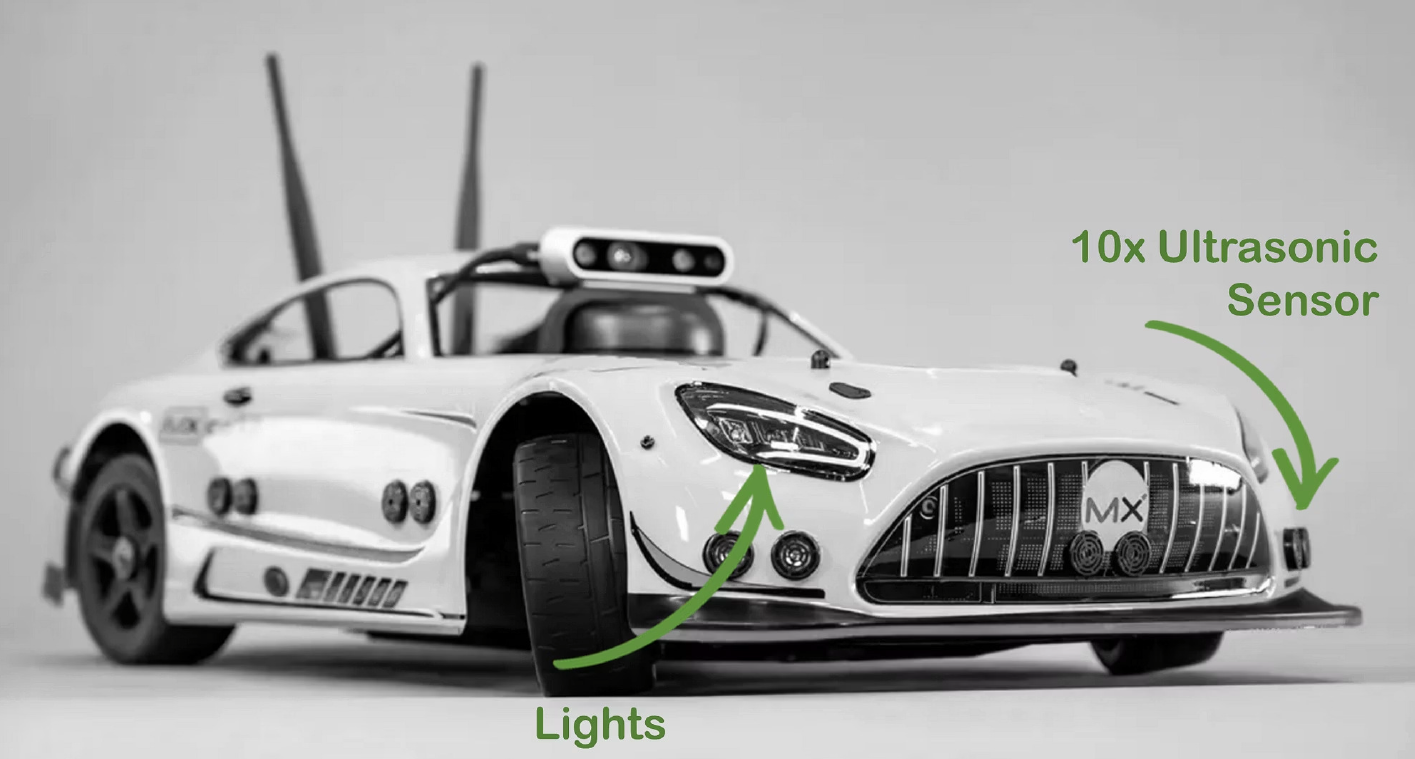
\includegraphics[
    width=7.02in
]{AV4of5.png}
};

% tight green banner on hero
\node[
    anchor=south west,
    fill=DeepGreen,
    text=white,
    inner xsep=8pt,
    inner ysep=4.5pt,
    font=\sffamily\bfseries\fontsize{7.5}{6.5}\selectfont
]
at ($(current page.north west)+(0.64in,-2.72in)$)
{MXCARKIT AUTONOMOUS VEHICLE PLATFORM};

% Right-side project logic
\node[
    anchor=north west,
    text=PolyGold,
    font=\sffamily\bfseries\fontsize{8.2}{7.2}\selectfont
]
at ($(current page.north west)+(7.72in,-2.50in)$)
{PROJECT EVOLUTION};

\draw[DeepGreen,line width=1.0pt]
($(current page.north west)+(7.72in,-2.86in)$) --
($(current page.north west)+(10.54in,-2.86in)$);

\foreach \y/\num/\ttl/\sub in {
3.14/01/PLATFORM/Camera + embedded compute,
3.68/02/BASELINE/Canny edges + pixel windows,
4.22/03/DIAGNOSIS/Noise + viewpoint failures,
4.76/04/REFINEMENT/Left-right lane evidence,
5.30/05/CONTROL/FSM + PD steering
}{
\node[
    anchor=north west,
    align=left,
    text width=2.55in
]
at ($(current page.north west)+(7.72in,-\y in)$)
{
{\textcolor{PolyGold}{\sffamily\bfseries\fontsize{7.1}{6.2}\selectfont \num}}
\hspace{5pt}
{\textcolor{DeepGreen}{\sffamily\bfseries\fontsize{7.4}{6.5}\selectfont \ttl}}\\[2pt]
{\textcolor{Muted}{\sffamily\fontsize{8.0}{5.5}\selectfont \sub}}
};
}

% bottom project summary band
\fill[SoftGreen,rounded corners=3pt]
($(current page.north west)+(0.46in,-6.48in)$)
rectangle
($(current page.north west)+(10.54in,-7.92in)$);

\node[
    anchor=north west,
    text=DeepGreen,
    font=\sffamily\bfseries\fontsize{8.1}{7.2}\selectfont
]
at ($(current page.north west)+(0.72in,-6.73in)$)
{DEVELOPMENT STACK};

\node[
    anchor=north west,
    align=left,
    text width=9.55in,
    font=\fontsize{7.4}{7.0}\selectfont,
    text=Ink
]
at ($(current page.north west)+(0.72in,-7.09in)$)
{
\textbf{Python} for perception and control development,
\textbf{Google Colab} for offline image/data analysis, and
\textbf{Foxglove} for inspection and visualization of recorded robotics data.
The final controller combined visual lane information with discrete road
states and closed-loop steering commands.
};

\RFFooter
{\hyperlink{autonomy}{\faArrowLeft\ AUTONOMY}}
{1 / 8}
{\hyperlink{roadfollowing-platform}{PLATFORM \faArrowRight}}

\end{tikzpicture}


%==============================================================
% PAGE 11B — LEARNING PLATFORM
%==============================================================

\clearpage
\thispagestyle{empty}
\hypertarget{roadfollowing-platform}{}
\null

\begin{tikzpicture}[remember picture,overlay]

\RFPageBase
\RFHeader
{LEARNING PLATFORM}
{THE AUTONOMOUS-VEHICLE HARDWARE STACK}
{Compute, perception, low-level I/O, vehicle power, and actuation architecture}

% Dense 2x2 image mosaic with tight spacing
\node[anchor=north west,inner sep=0pt]
at ($(current page.north west)+(0.94in,-1.68in)$)
{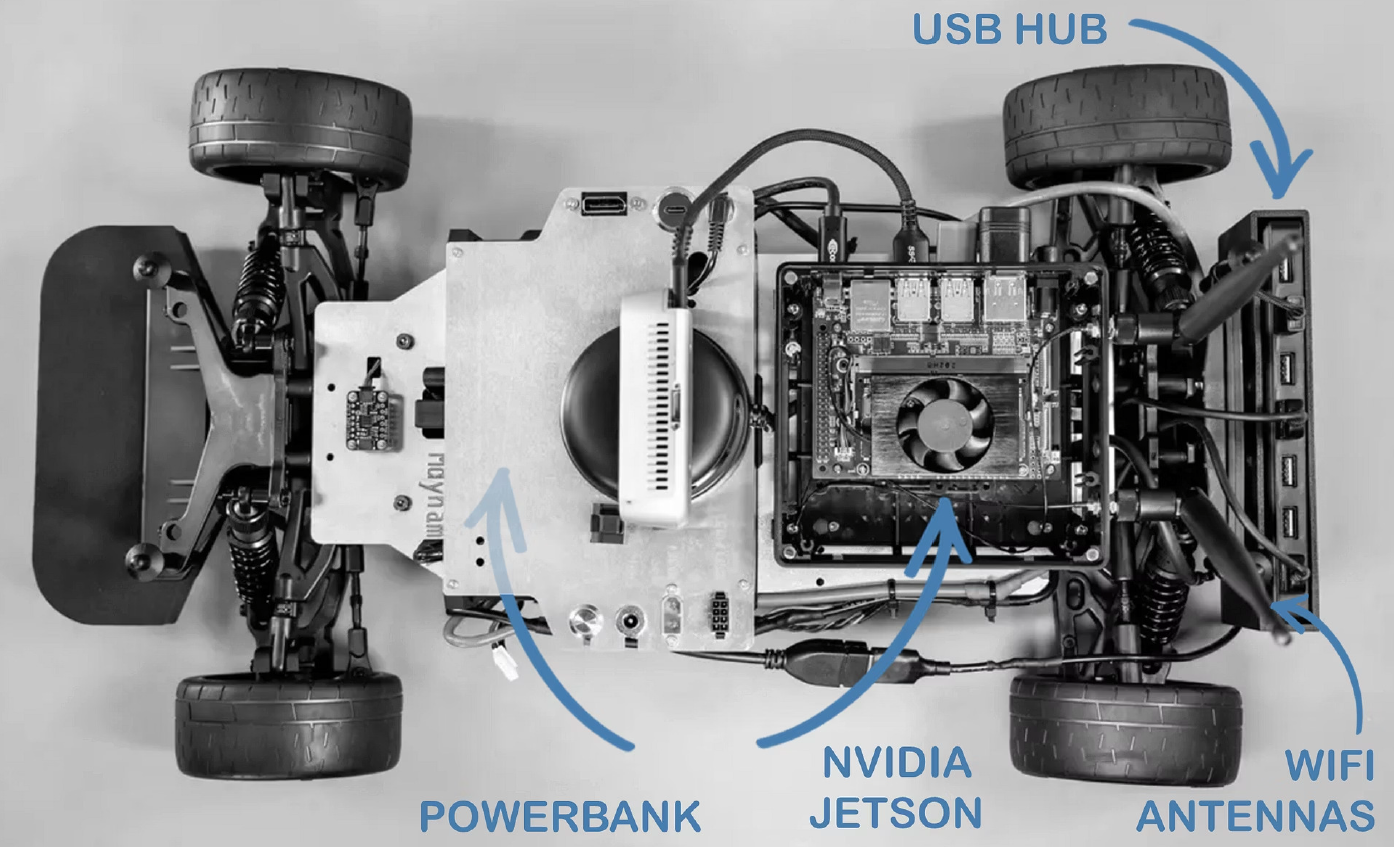
\includegraphics[width=4.52in]{AV1of5.png}};

\node[
    anchor=north west,
    fill=DeepGreen,
    text=white,
    inner xsep=7pt,
    inner ysep=4pt,
    font=\sffamily\bfseries\fontsize{7.2}{6.2}\selectfont
]
at ($(current page.north west)+(1.06in,-1.81in)$)
{COMPUTE + NETWORK};

\node[anchor=north west,inner sep=0pt]
at ($(current page.north west)+(5.54in,-1.68in)$)
{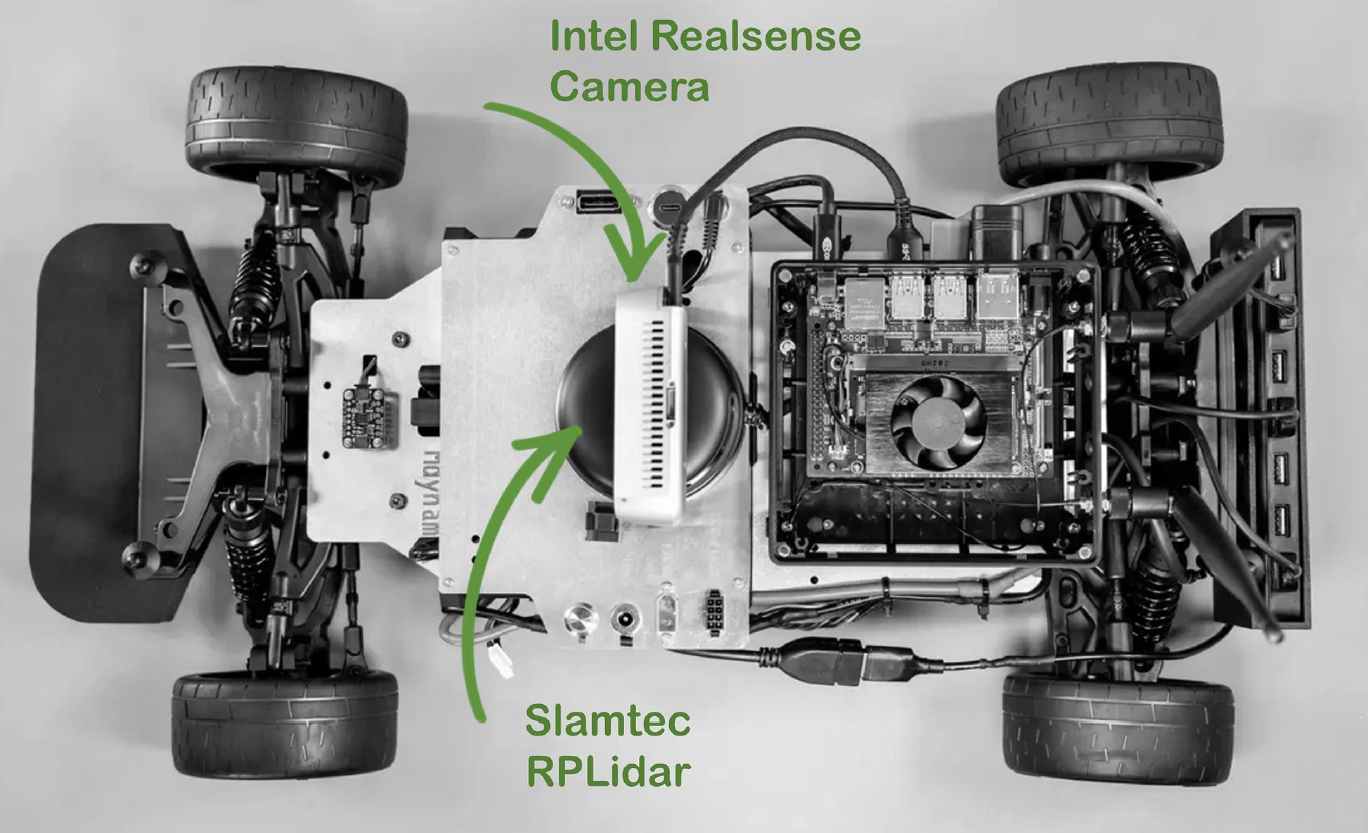
\includegraphics[width=4.52in]{AV2of5.png}};

\node[
    anchor=north west,
    fill=DeepGreen,
    text=white,
    inner xsep=7pt,
    inner ysep=4pt,
    font=\sffamily\bfseries\fontsize{7.2}{6.2}\selectfont
]
at ($(current page.north west)+(5.66in,-1.81in)$)
{FORWARD PERCEPTION};

\node[anchor=north west,inner sep=0pt]
at ($(current page.north west)+(0.94in,-4.53in)$)
{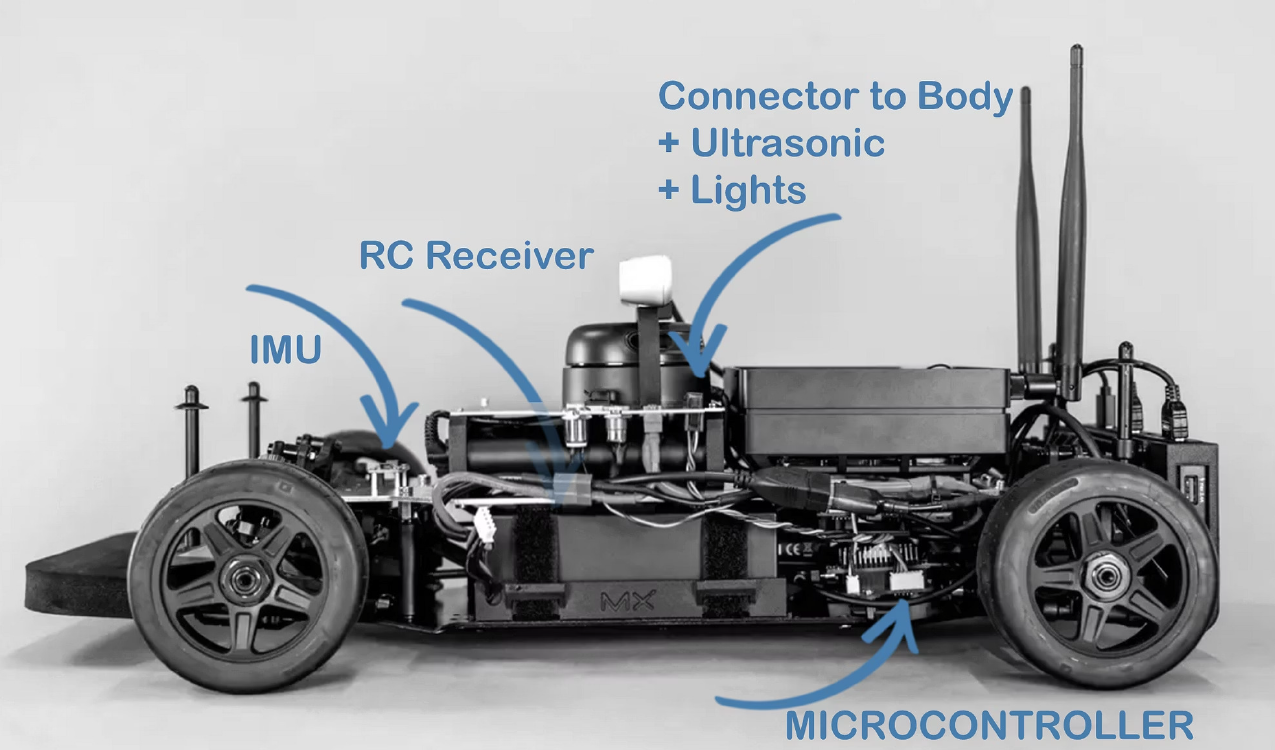
\includegraphics[width=4.52in]{AV3of5.png}};

\node[
    anchor=north west,
    fill=DeepGreen,
    text=white,
    inner xsep=7pt,
    inner ysep=4pt,
    font=\sffamily\bfseries\fontsize{7.2}{6.2}\selectfont
]
at ($(current page.north west)+(1.06in,-4.66in)$)
{LOW-LEVEL I/O};

\node[anchor=north west,inner sep=0pt]
at ($(current page.north west)+(5.54in,-4.53in)$)
{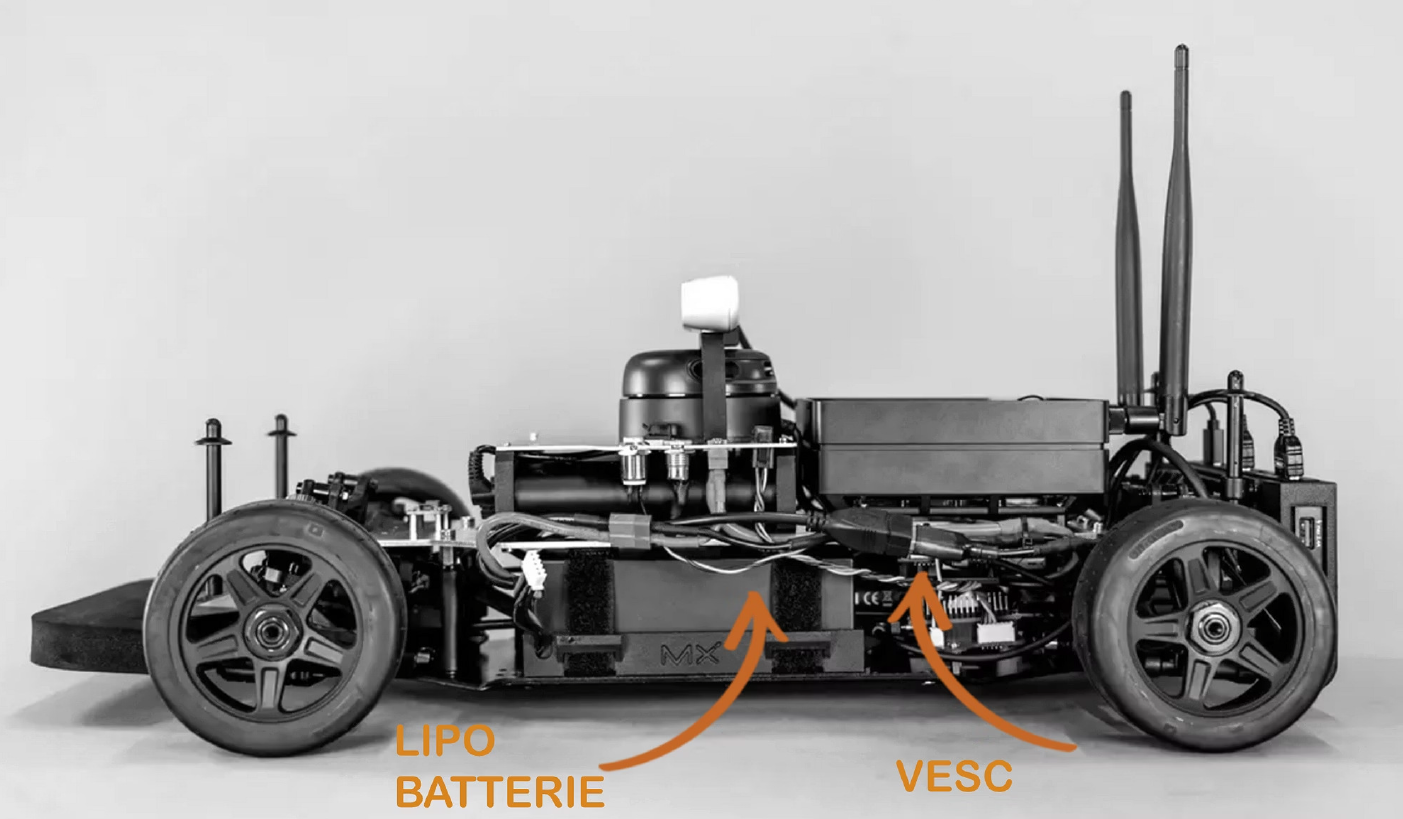
\includegraphics[width=4.52in]{AV5of5.png}};

\node[
    anchor=north west,
    fill=DeepGreen,
    text=white,
    inner xsep=7pt,
    inner ysep=4pt,
    font=\sffamily\bfseries\fontsize{7.2}{6.2}\selectfont
]
at ($(current page.north west)+(5.66in,-4.66in)$)
{POWER + ACTUATION};

% compact summary and architecture strip
\draw[RuleGray,line width=0.55pt]
($(current page.north west)+(0.46in,-7.27in)$) --
($(current page.north west)+(10.54in,-7.27in)$);

\node[
    anchor=north west,
    text=DeepGreen,
    font=\sffamily\bfseries\fontsize{8.0}{7.1}\selectfont
]
at ($(current page.north west)+(0.46in,-7.35in)$)
{ROAD-FOLLOWER SIGNAL PATH};

\node[
    anchor=north west,
    align=center,
    text width=10.08in,
    font=\sffamily\bfseries\fontsize{7.7}{7.3}\selectfont,
    text=DeepGreen
]
at ($(current page.north west)+(0.46in,-7.7in)$)
{
\textbf{INTEL REALSENSE}
\hspace{7pt}$\rightarrow$\hspace{7pt}
\textbf{NVIDIA JETSON / PYTHON}
\hspace{7pt}$\rightarrow$\hspace{7pt}
PERCEPTION LOGIC
\hspace{7pt}$\rightarrow$\hspace{7pt}
STEERING COMMAND
};


\RFFooter
{\hyperlink{roadfollowing}{\faArrowLeft\ OVERVIEW}}
{2 / 8}
{\hyperlink{roadfollowing-canny}{INITIAL PERCEPTION \faArrowRight}}

\end{tikzpicture}


%==============================================================
% PAGE 11C — CANNY EDGE BASELINE
%==============================================================

\clearpage
\thispagestyle{empty}
\hypertarget{roadfollowing-canny}{}
\null

\begin{tikzpicture}[remember picture,overlay]

\RFPageBase
\RFHeader
{PERCEPTION DEVELOPMENT}
{FINDING THE ROAD WITH EDGES}
{Baseline vision pipeline
\hspace{7pt}\textbullet\hspace{7pt}
\textbf{Python} + \textbf{Google Colab}
\hspace{7pt}\textbullet\hspace{7pt}
Canny edge detection + ROI tuning}

% Narrative setup
\node[
    anchor=north west,
    align=left,
    text width=10.00in,
    font=\fontsize{8.0}{9.4}\selectfont,
    text=Ink
]
at ($(current page.north west)+(0.46in,-1.60in)$)
{
The first road-following strategy reduced each camera frame to a simpler
question: \textbf{where are the strongest track-boundary edges?} The image
was preprocessed, converted to Canny edges, masked to a smaller region of
interest, and then summarized by the number of usable white pixels inside
that window. This provided a fast baseline that could be tuned on recorded
frames before returning to the physical vehicle.
};

% Pipeline band
\node[
    anchor=north west,
    text=DeepGreen,
    font=\sffamily\bfseries\fontsize{8.1}{9.0}\selectfont
]
at ($(current page.north west)+(0.46in,-2.28in)$)
{BASELINE PERCEPTION PIPELINE};

\foreach \x/\ttl/\sub in {
0.46/CAMERA/Raw frame,
2.56/PREPROCESS/Blur + mask,
4.66/CANNY/Extract edges,
6.76/ROI/Count lane pixels,
8.86/STEERING/Use visual error
}{
\node[
    anchor=north west,
    draw=DeepGreen,
    rounded corners=2pt,
    line width=0.60pt,
    minimum width=1.68in,
    minimum height=0.66in,
    align=center,
    text=DeepGreen
]
at ($(current page.north west)+(\x in,-2.55in)$)
{
{\sffamily\bfseries\fontsize{6.7}{7.4}\selectfont \ttl}\\[1pt]
{\sffamily\fontsize{6.2}{7.0}\selectfont \sub}
};
}

\foreach \xa/\xb in {2.16/2.51,4.26/4.61,6.36/6.71,8.46/8.81}{
\draw[->,PolyGold,line width=1.0pt]
($(current page.north west)+(\xa in,-2.88in)$) --
($(current page.north west)+(\xb in,-2.88in)$);
}

% Main processing figure, full width and easy to read
\node[
    anchor=north west,
    inner sep=0pt,
    draw=DeepGreen,
    line width=0.55pt
]
at ($(current page.north west)+(0.46in,-3.28in)$)
{
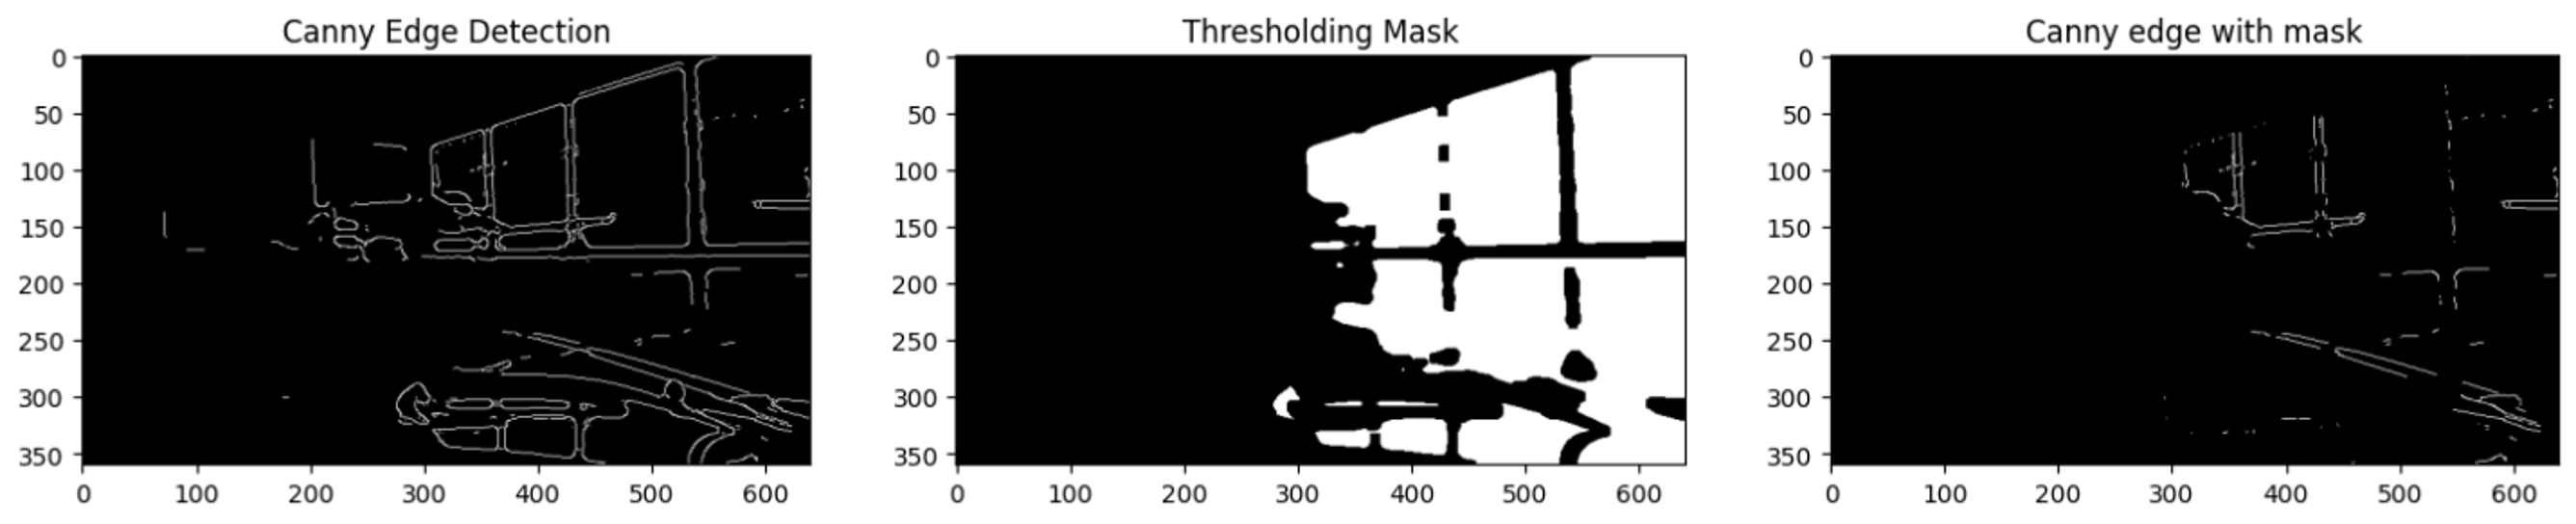
\includegraphics[width=10.08in]{CannyEdgeDetectionMethod.png}
};

% Larger baseline explanation, kept directly beneath the figure
\draw[RuleGray,line width=0.45pt]
($(current page.north west)+(0.46in,-5.13in)$) --
($(current page.north west)+(10.54in,-5.13in)$);

\node[
    anchor=north west,
    text=DeepGreen,
    font=\sffamily\bfseries\fontsize{8.4}{9.2}\selectfont
]
at ($(current page.north west)+(0.46in,-5.34in)$)
{WHAT THE BASELINE WAS DOING};

\node[
    anchor=north west,
    align=left,
    text width=10.00in,
    font=\fontsize{8.0}{9.35}\selectfont,
    text=Ink
]
at ($(current page.north west)+(0.46in,-5.62in)$)
{
Canny edge detection exposed high-contrast structure, while thresholding and
masking suppressed much of the surrounding scene. The controller then evaluated
a deliberately constrained road region instead of reacting to every visible edge.
This converted each camera frame into a lightweight visual signal that could be
tested and tuned rapidly on recorded data before returning to the vehicle.
};

% Compact transition narrative
\node[
    anchor=north west,
    text=DeepGreen,
    font=\sffamily\bfseries\fontsize{8.1}{9.0}\selectfont
]
at ($(current page.north west)+(0.46in,-6.48in)$)
{WHY A SEPARATE TUNING STUDY WAS NEEDED};

\node[
    anchor=north west,
    align=left,
    text width=10.00in,
    font=\fontsize{7.65}{8.9}\selectfont,
    text=Ink
]
at ($(current page.north west)+(0.46in,-6.78in)$)
{
Lighting, viewpoint, curvature, and background clutter changed the detector response
from frame to frame. The next step therefore compared representative scenes and
preprocessing settings side-by-side rather than selecting parameters from one image.
};


% RESOURCE BAR — formatted consistently with the rest of the portfolio
\fill[SoftGreen!34,rounded corners=4pt]
($(current page.south west)+(0.46in,0.58in)$)
rectangle
($(current page.south east)+(-0.46in,1.08in)$);

\draw[RuleGray,line width=0.45pt,rounded corners=4pt]
($(current page.south west)+(0.46in,0.58in)$)
rectangle
($(current page.south east)+(-0.46in,1.08in)$);

\node[
    anchor=center,
    text=DeepGreen,
    font=\sffamily\bfseries\fontsize{6.9}{7.7}\selectfont,
    align=center
]
at ($(current page.south)+(0,0.83in)$)
{
\href{https://drive.google.com/file/d/11rblY0SEngrENpYdcI8bonIHuGg9S97w/view?usp=drive_link}
{\faPlayCircle\ STATIONARY REMOTE-CONTROLLED DEMO}
\hspace{18pt}
\faFilePdf\ PROJECT MEMO
\hspace{18pt}
\faCode\ COLAB / GITHUB
};

\RFFooter
{\hyperlink{roadfollowing-platform}{\faArrowLeft\ PLATFORM}}
{3 / 9}
{\hyperlink{roadfollowing-tuning}{DETECTOR TUNING \faArrowRight}}

\end{tikzpicture}


%==============================================================

%==============================================================
% PAGE 11D — DETECTOR TUNING STUDY
%==============================================================

\clearpage
\thispagestyle{empty}
\hypertarget{roadfollowing-tuning}{}
\null

\begin{tikzpicture}[remember picture,overlay]

\RFPageBase
\RFHeader
{DETECTOR TUNING}
{TUNING THE DETECTOR ACROSS REPRESENTATIVE FRAMES}
{Parameter exploration
\hspace{7pt}\textbullet\hspace{7pt}
Canny thresholds
\hspace{7pt}\textbullet\hspace{7pt}
blur strategy
\hspace{7pt}\textbullet\hspace{7pt}
ROI robustness}

% Narrative setup
\node[
    anchor=north west,
    align=left,
    text width=10.00in,
    font=\fontsize{7.5}{8.9}\selectfont,
    text=Ink
]
at ($(current page.north west)+(0.46in,-1.72in)$)
{
A detector that looked acceptable in one image could fail a few moments later.
To avoid tuning by intuition alone, representative frames from different
sections of the course were processed under several combinations of
\textbf{Canny thresholds}, \textbf{blur methods}, and \textbf{kernel sizes}.
The goal was to identify settings that preserved the painted lane boundary
without amplifying background edges.
};

% Key-frames tuning comparison — scaled down, centered, and shifted upward
\node[
    anchor=north,
    inner sep=0pt,
    draw=DeepGreen,
    line width=0.75pt
]
at ($(current page.north)+(0,-2.36in)$)
{
\includegraphics[
    width=7.70in,
    keepaspectratio
]{KeyFramesVSsettings.png}
};

\node[
    anchor=north west,
    fill=DeepGreen,
    text=white,
    inner xsep=8pt,
    inner ysep=4.5pt,
    font=\sffamily\bfseries\fontsize{6.2}{6.9}\selectfont
]
at ($(current page.north west)+(1.82in,-2.55in)$)
{SIDE-BY-SIDE PARAMETER EXPLORATION};

% Bottom interpretation area
\draw[RuleGray,line width=0.6pt]
($(current page.north west)+(0.46in,-6.95in)$) --
($(current page.north west)+(10.54in,-6.95in)$);

\node[
    anchor=north west,
    text=DeepGreen,
    font=\sffamily\bfseries\fontsize{8.0}{8.8}\selectfont
]
at ($(current page.north west)+(0.46in,-7.22in)$)
{WHAT THE COMPARISON REVEALED};

\node[
    anchor=north west,
    align=left,
    text width=4.78in,
    font=\fontsize{7.0}{8.3}\selectfont,
    text=Ink
]
at ($(current page.north west)+(0.46in,-7.58in)$)
{
\textbf{\textcolor{PolyGold}{1. Sensitivity to thresholds}}\\[3pt]
Lower thresholds exposed more edges, but also admitted more background
structure. Higher thresholds reduced clutter but could erase faint lane
features.
};

\node[
    anchor=north west,
    align=left,
    text width=4.78in,
    font=\fontsize{7.0}{8.3}\selectfont,
    text=Ink
]
at ($(current page.north west)+(5.76in,-7.58in)$)
{
\textbf{\textcolor{PolyGold}{2. Preprocessing mattered}}\\[3pt]
Blur method and kernel size changed which boundaries survived into the Canny
image. The comparison showed that detector quality depended on the whole
preprocessing chain, not one threshold in isolation.
};


\RFFooter
{\hyperlink{roadfollowing-canny}{\faArrowLeft\ CANNY BASELINE}}
{4 / 9}
{\hyperlink{roadfollowing-failure}{FAILURE ANALYSIS \faArrowRight}}

\end{tikzpicture}


% PAGE 11D — FAILURE ANALYSIS
%==============================================================

\clearpage
\thispagestyle{empty}
\hypertarget{roadfollowing-failure}{}
\null

\begin{tikzpicture}[remember picture,overlay]

\RFPageBase
\RFHeader
{PERCEPTION DIAGNOSIS}
{WHEN THE PIXEL COUNT LIED}
{Failure modes in recorded frames \hspace{7pt}\textbullet\hspace{7pt}
scene clutter \hspace{7pt}\textbullet\hspace{7pt}
viewpoint sensitivity}

% histogram dominates top-left
\node[anchor=north west,inner sep=0pt]
at ($(current page.north west)+(0.46in,-1.75in)$)
{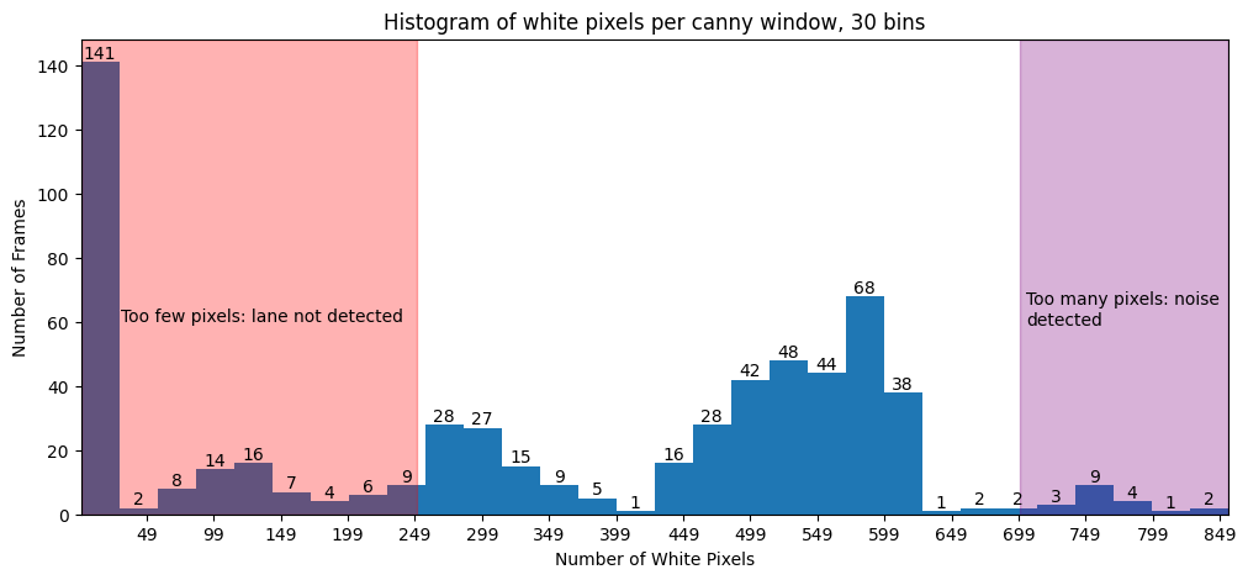
\includegraphics[width=5.92in,height=3.00in,keepaspectratio]{BadAlgorithmHistogram.png}};

% high-count example top-right
\node[anchor=north west,inner sep=0pt]
at ($(current page.north west)+(6.66in,-1.75in)$)
{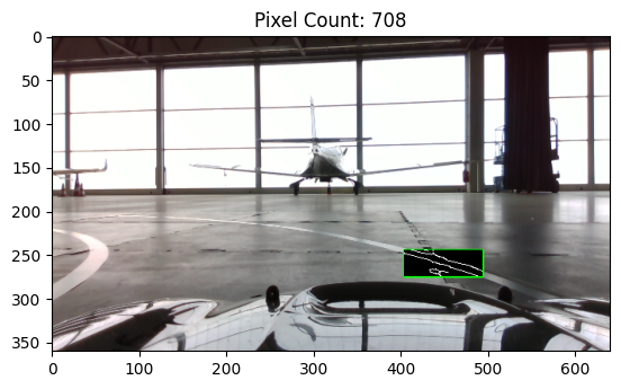
\includegraphics[width=3.88in,height=2.05in,keepaspectratio]{HighPixelCountFrame.png}};

\node[
    anchor=north west,
    align=left,
    text width=3.82in,
    font=\fontsize{7.05}{6.55}\selectfont,
    text=Ink
]
at ($(current page.north west)+(6.66in,-3.92in)$)
{
A high edge count did not automatically mean the lane was well detected.
Background geometry, reflections, and unrelated high-contrast objects could
inflate the measurement.
};

% lower visual pair
\draw[RuleGray,line width=0.55pt]
($(current page.north west)+(0.46in,-4.51in)$) --
($(current page.north west)+(10.54in,-4.51in)$);

\node[
    anchor=north west,
    text=DeepGreen,
    font=\sffamily\bfseries\fontsize{8.3}{7.4}\selectfont
]
at ($(current page.north west)+(0.46in,-4.77in)$)
{NOISE + VIEWPOINT EFFECTS};

\node[anchor=north west,inner sep=0pt]
at ($(current page.north west)+(0.46in,-5.11in)$)
{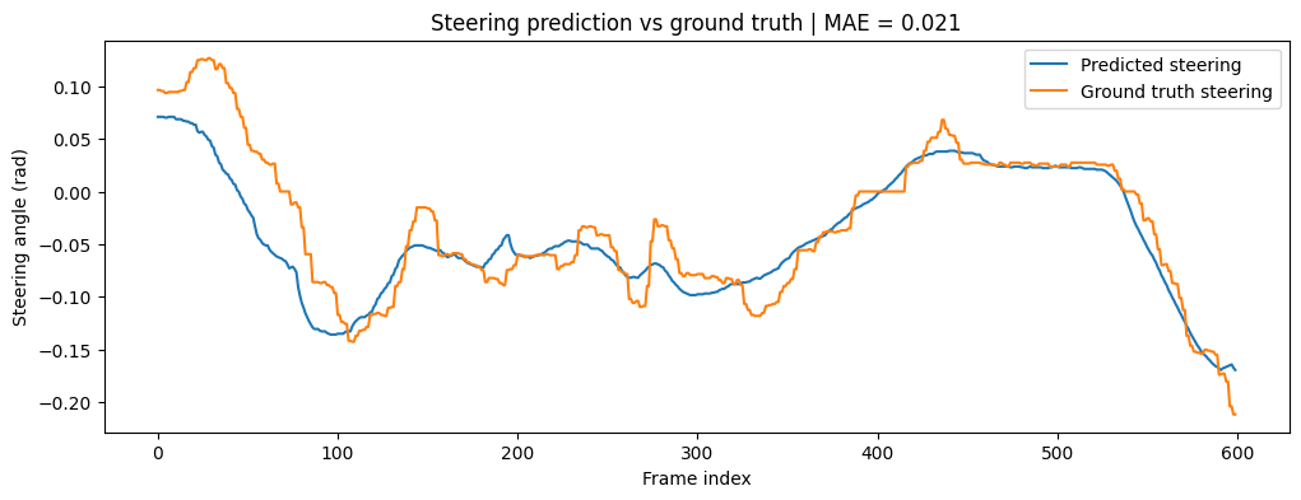
\includegraphics[width=5.02in,height=2.10in,keepaspectratio]{CannyEdgePlotNoiseDemo.png}};

\node[anchor=north west,inner sep=0pt]
at ($(current page.north west)+(5.76in,-5.11in)$)
{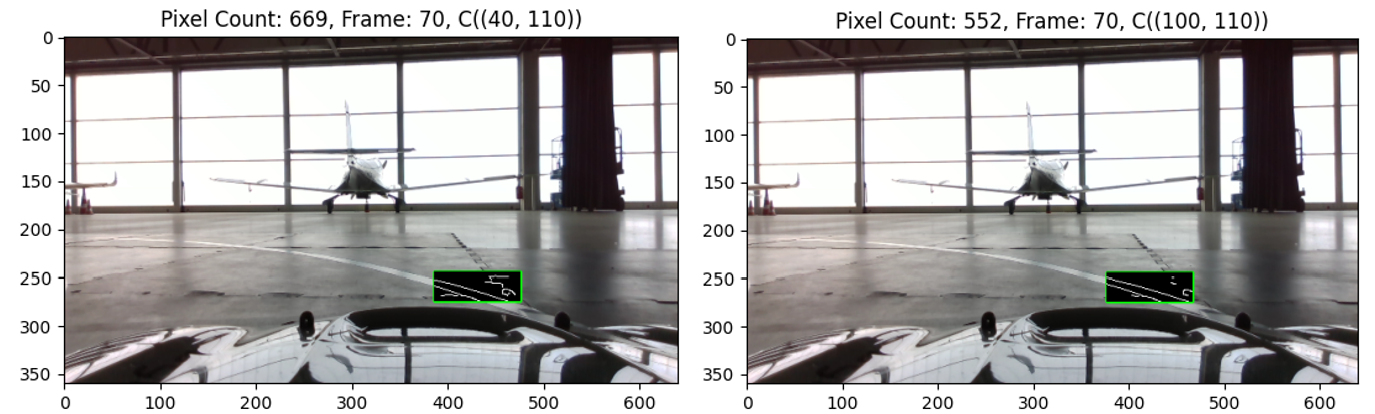
\includegraphics[width=4.78in,height=2.10in,keepaspectratio]{staticVSdynamicPxlCnt.png}};

% design lesson strip
\fill[SoftGold,rounded corners=3pt]
($(current page.north west)+(0.46in,-7.27in)$)
rectangle
($(current page.north west)+(10.54in,-7.92in)$);

\fill[PolyGold]
($(current page.north west)+(0.46in,-7.27in)$)
rectangle
($(current page.north west)+(0.56in,-7.92in)$);

\node[
    anchor=west,
    align=left,
    text width=9.48in,
    font=\sffamily\fontsize{7.3}{6.8}\selectfont,
    text=Ink
]
at ($(current page.north west)+(0.76in,-7.595in)$)
{
\textbf{\textcolor{DeepGreen}{DESIGN LESSON}}
\hspace{8pt}
A single raw edge count mixed perception and control too closely. The next
design needed to answer a cleaner question:
\textbf{which lane boundary is actually visible?}
};

\RFFooter
{\hyperlink{roadfollowing-canny}{\faArrowLeft\ INITIAL PERCEPTION}}
{5 / 9}
{\hyperlink{roadfollowing-dynamic}{REFINED DETECTOR \faArrowRight}}

\end{tikzpicture}


%==============================================================
% PAGE 11E — DYNAMIC DETECTOR
%==============================================================

\clearpage
\thispagestyle{empty}
\hypertarget{roadfollowing-dynamic}{}
\null

\begin{tikzpicture}[remember picture,overlay]

\RFPageBase
\RFHeader
{PERCEPTION REFINEMENT}
{FROM STATIC WINDOW TO DYNAMIC LANE EVIDENCE}
{Dynamic region-of-interest logic \hspace{7pt}\textbullet\hspace{7pt}
pixel-count thresholds \hspace{7pt}\textbullet\hspace{7pt}
left/right detection flags}

% top image comparison
\node[anchor=north west,inner sep=0pt]
at ($(current page.north west)+(0.46in,-1.76in)$)
{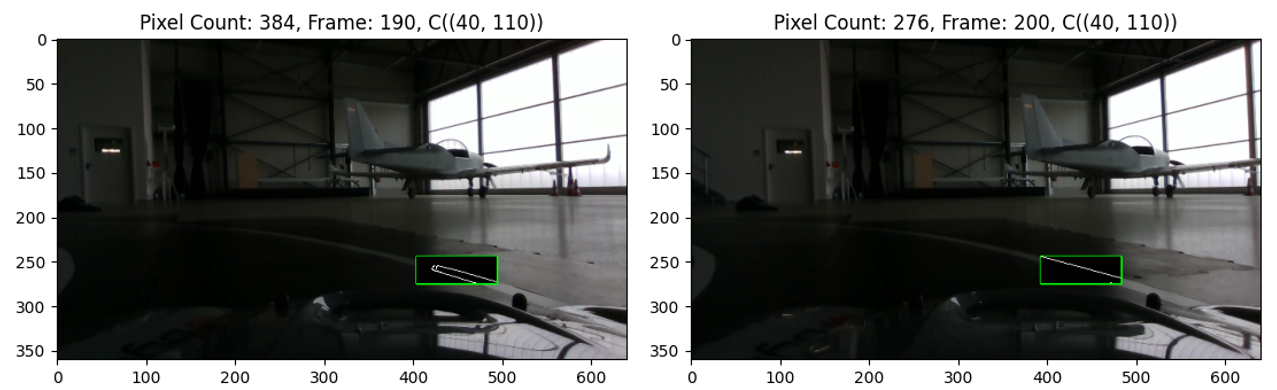
\includegraphics[width=4.90in,height=2.14in,keepaspectratio]{Static_Canny_Detection.png}};

\node[
    anchor=north west,
    fill=DeepGreen,
    text=white,
    inner xsep=7pt,
    inner ysep=4pt,
    font=\sffamily\bfseries\fontsize{6.9}{5.9}\selectfont
]
at ($(current page.north west)+(0.58in,-1.89in)$)
{STATIC DETECTION WINDOW};

\node[anchor=north west,inner sep=0pt]
at ($(current page.north west)+(5.64in,-1.76in)$)
{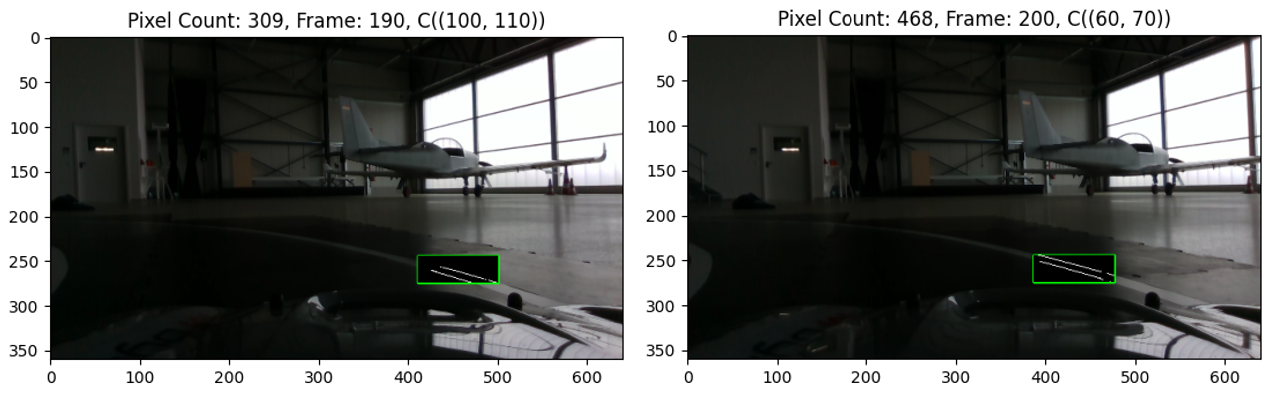
\includegraphics[width=4.90in,height=2.14in,keepaspectratio]{Dynamic_Canny_Detection.png}};

\node[
    anchor=north west,
    fill=DeepGreen,
    text=white,
    inner xsep=7pt,
    inner ysep=4pt,
    font=\sffamily\bfseries\fontsize{6.9}{5.9}\selectfont
]
at ($(current page.north west)+(5.76in,-1.89in)$)
{DYNAMIC DETECTION WINDOW};

% mid histograms
\node[
    anchor=north west,
    text=DeepGreen,
    font=\sffamily\bfseries\fontsize{8.3}{7.4}\selectfont
]
at ($(current page.north west)+(0.46in,-4.13in)$)
{AFTER REFINEMENT};

\node[anchor=north west,inner sep=0pt]
at ($(current page.north west)+(0.46in,-4.46in)$)
{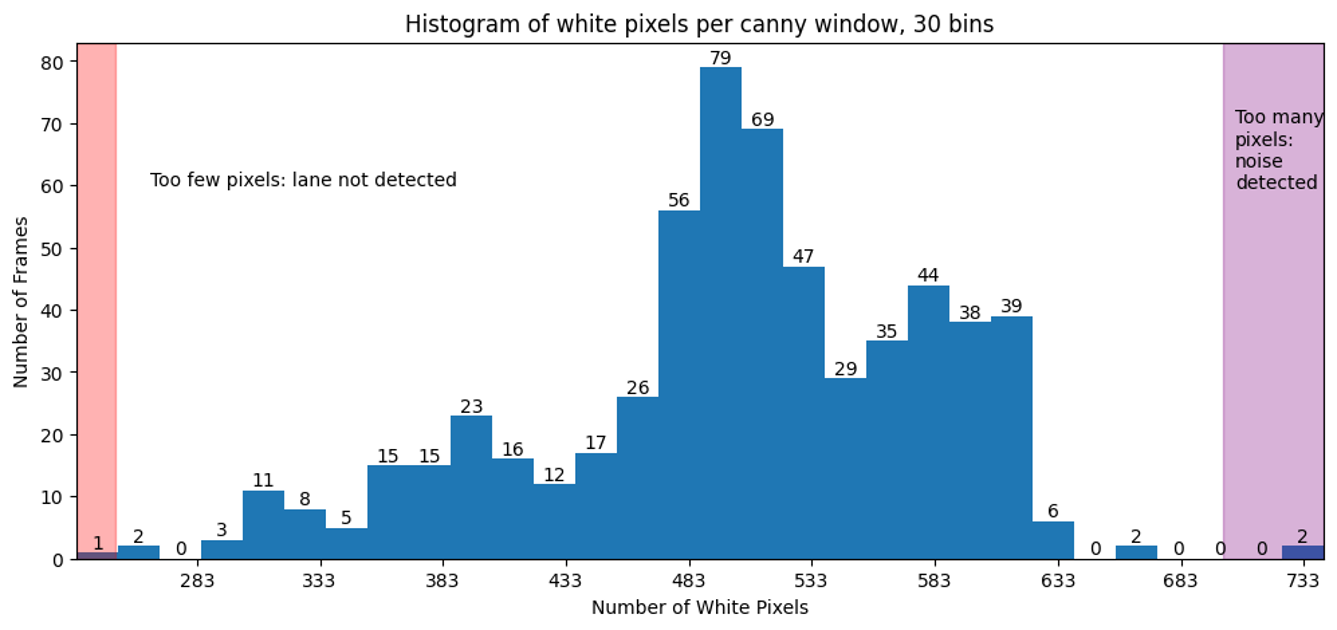
\includegraphics[width=4.90in,height=2.30in,keepaspectratio]{DynamicCannyHistogram.png}};

\node[anchor=north west,inner sep=0pt]
at ($(current page.north west)+(5.64in,-4.46in)$)
{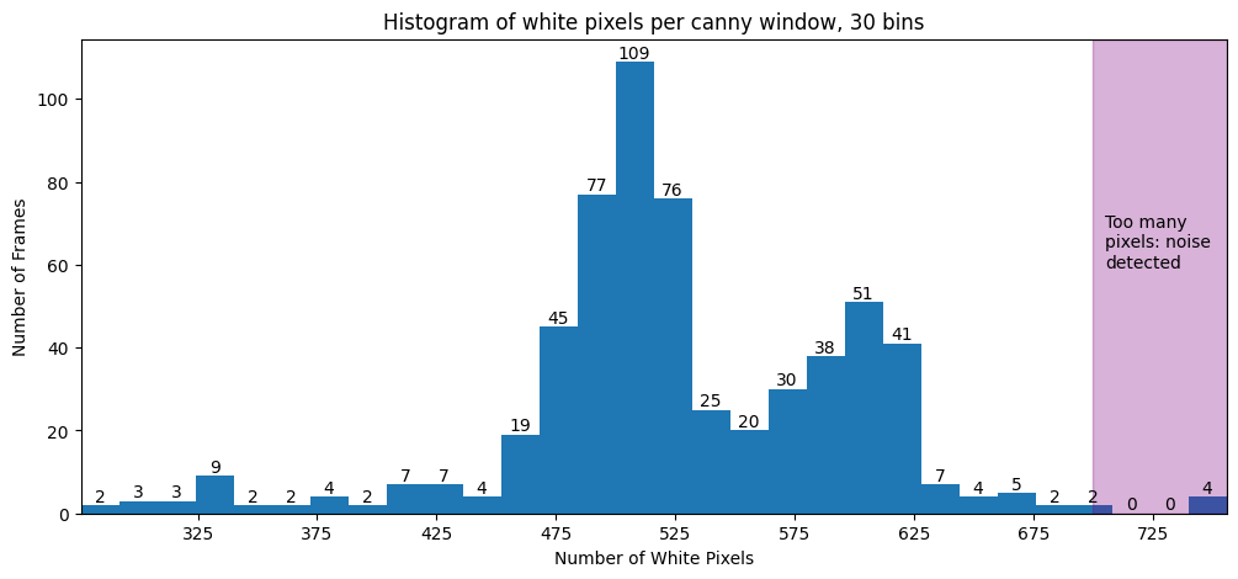
\includegraphics[width=4.90in,height=2.30in,keepaspectratio]{GoodAlgorithmHistogram.png}};

% bottom explanation
\node[
    anchor=north west,
    align=left,
    text width=4.82in,
    font=\fontsize{7.1}{6.6}\selectfont,
    text=Ink
]
at ($(current page.north west)+(0.46in,-6.94in)$)
{
The refined detector produced a more useful distribution. Pixel-count
thresholds could now be interpreted as \textbf{lane evidence} instead of as a
direct steering command.
};

\node[
    anchor=north west,
    align=left,
    text width=4.82in,
    font=\fontsize{7.1}{6.6}\selectfont,
    text=Ink
]
at ($(current page.north west)+(5.64in,-6.94in)$)
{
The output became two explicit variables:
\texttt{LINE\_LEFT\_DETECTED} and
\texttt{LINE\_RIGHT\_DETECTED}. These flags formed the interface between
perception and the state machine.
};

\fill[DeepGreen,rounded corners=3pt]
($(current page.north west)+(0.46in,-7.72in)$)
rectangle
($(current page.north west)+(10.54in,-8.in)$);

\node[
    anchor=center,
    text=white,
    font=\sffamily\bfseries\fontsize{7.5}{7.0}\selectfont
]
at ($(current page.north west)+(5.50in,-7.85in)$)
{
RAW PIXELS
\hspace{8pt}$\rightarrow$\hspace{8pt}
LANE EVIDENCE
\hspace{8pt}$\rightarrow$\hspace{8pt}
ROAD STATE
};

\RFFooter
{\hyperlink{roadfollowing-failure}{\faArrowLeft\ FAILURE ANALYSIS}}
{6 / 9}
{\hyperlink{roadfollowing-state}{ROAD STATE \faArrowRight}}

\end{tikzpicture}


%==============================================================
% PAGE 11F — ROAD STATE REPRESENTATION
%==============================================================

\clearpage
\thispagestyle{empty}
\hypertarget{roadfollowing-state}{}
\null

\begin{tikzpicture}[remember picture,overlay]

\RFPageBase
\RFHeader
{ROAD-STATE REPRESENTATION}
{TURNING LANE EVIDENCE INTO A DRIVING CONDITION}
{Left/right lane segmentation \hspace{7pt}\textbullet\hspace{7pt}
road geometry inference \hspace{7pt}\textbullet\hspace{7pt}
FSM transition evidence}

% hero state-transition image — very tight green border
\node[
    anchor=north west,
    inner sep=0pt,
    draw=DeepGreen,
    line width=0.65pt
]
at ($(current page.north west)+(0.46in,-1.76in)$)
{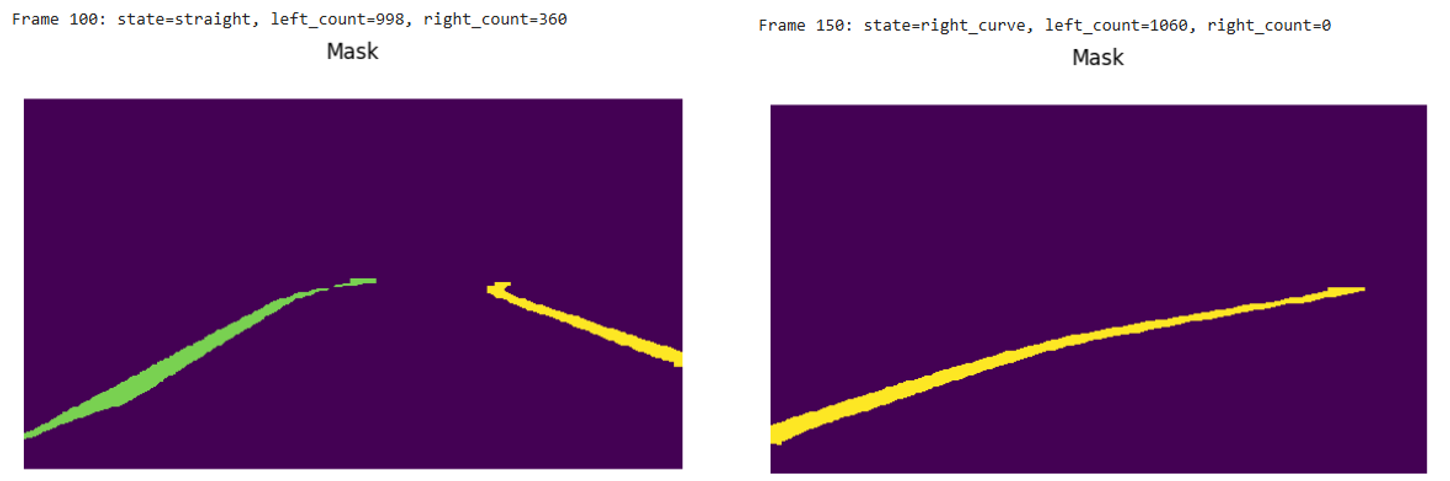
\includegraphics[width=10.08in,height=3.30in,keepaspectratio]{state_transition.png}};

% tight banner — shifted upward toward the top of the image
\node[
    anchor=south west,
    fill=DeepGreen,
    text=white,
    inner xsep=8pt,
    inner ysep=4pt,
    font=\sffamily\bfseries\fontsize{7.0}{6.1}\selectfont
]
at ($(current page.north west)+(0.60in,-2.62in)$)
{LEFT / RIGHT LANE REPRESENTATION};

% explanatory split
\node[
    anchor=north west,
    align=left,
    text width=4.85in,
    font=\fontsize{7.2}{6.75}\selectfont,
    text=Ink
]
at ($(current page.north west)+(0.46in,-5.36in)$)
{
In a straight segment, both painted boundaries can be visible. During a
right-hand curve, the right boundary can disappear from the usable image
region while the left remains visible; the inverse occurs during a left-hand
curve.
};

\node[
    anchor=north west,
    text=PolyGold,
    font=\sffamily\bfseries\fontsize{7.6}{6.7}\selectfont
]
at ($(current page.north west)+(5.76in,-5.36in)$)
{PERCEPTION FLAGS};

\node[
    anchor=north west,
    align=left,
    text width=4.40in,
    font=\ttfamily\fontsize{7.3}{6.9}\selectfont,
    text=DeepGreen
]
at ($(current page.north west)+(5.76in,-5.70in)$)
{
LINE\_LEFT\_DETECTED\\
LINE\_RIGHT\_DETECTED\\
LINE\_LEFT\_MISSING\\
LINE\_RIGHT\_MISSING
};

% State preview row
\draw[RuleGray,line width=0.55pt]
($(current page.north west)+(0.46in,-6.40in)$) --
($(current page.north west)+(10.54in,-6.40in)$);

\node[
    anchor=north west,
    text=DeepGreen,
    font=\sffamily\bfseries\fontsize{8.3}{7.4}\selectfont
]
at ($(current page.north west)+(0.46in,-6.68in)$)
{THE THREE DRIVING CONDITIONS};

\foreach \x/\num/\ttl/\sub in {
0.46/01/STRAIGHT/Both lane boundaries available,
3.84/02/LEFT\_CURVE/Follow LINE\_RIGHT,
7.22/03/RIGHT\_CURVE/Follow LINE\_LEFT
}{
\node[
    anchor=north west,
    align=left,
    text width=3.42in
]
at ($(current page.north west)+(\x in,-7.10in)$)
{
{\textcolor{PolyGold}{\sffamily\bfseries\fontsize{7.1}{6.2}\selectfont \num}}\\[2pt]
{\textcolor{DeepGreen}{\sffamily\bfseries\fontsize{8.1}{7.2}\selectfont \ttl}}\\[3pt]
{\textcolor{Muted}{\sffamily\fontsize{8.1}{5.6}\selectfont \sub}}
};
}

\RFFooter
{\hyperlink{roadfollowing-dynamic}{\faArrowLeft\ REFINED DETECTOR}}
{7 / 9}
{\hyperlink{roadfollowing-fsm}{FSM + CONTROL \faArrowRight}}

\end{tikzpicture}


%==============================================================
% PAGE 11G — FSM + CONTROL
%==============================================================

\clearpage
\thispagestyle{empty}
\hypertarget{roadfollowing-fsm}{}
\null

\begin{tikzpicture}[remember picture,overlay]

\RFPageBase
\RFHeader
{AUTONOMOUS CONTROL}
{TURNING PERCEPTION INTO MOTION}
{Finite-state driving logic \hspace{7pt}\textbullet\hspace{7pt}
lane-reference selection \hspace{7pt}\textbullet\hspace{7pt}
PD steering response}

% FSM as hero
\node[
    anchor=north west,
    text=DeepGreen,
    font=\sffamily\bfseries\fontsize{8.3}{7.4}\selectfont
]
at ($(current page.north west)+(0.46in,-1.76in)$)
{FINITE-STATE DRIVING LOGIC};

\node[anchor=north west,inner sep=0pt]
at ($(current page.north west)+(0.46in,-2.10in)$)
{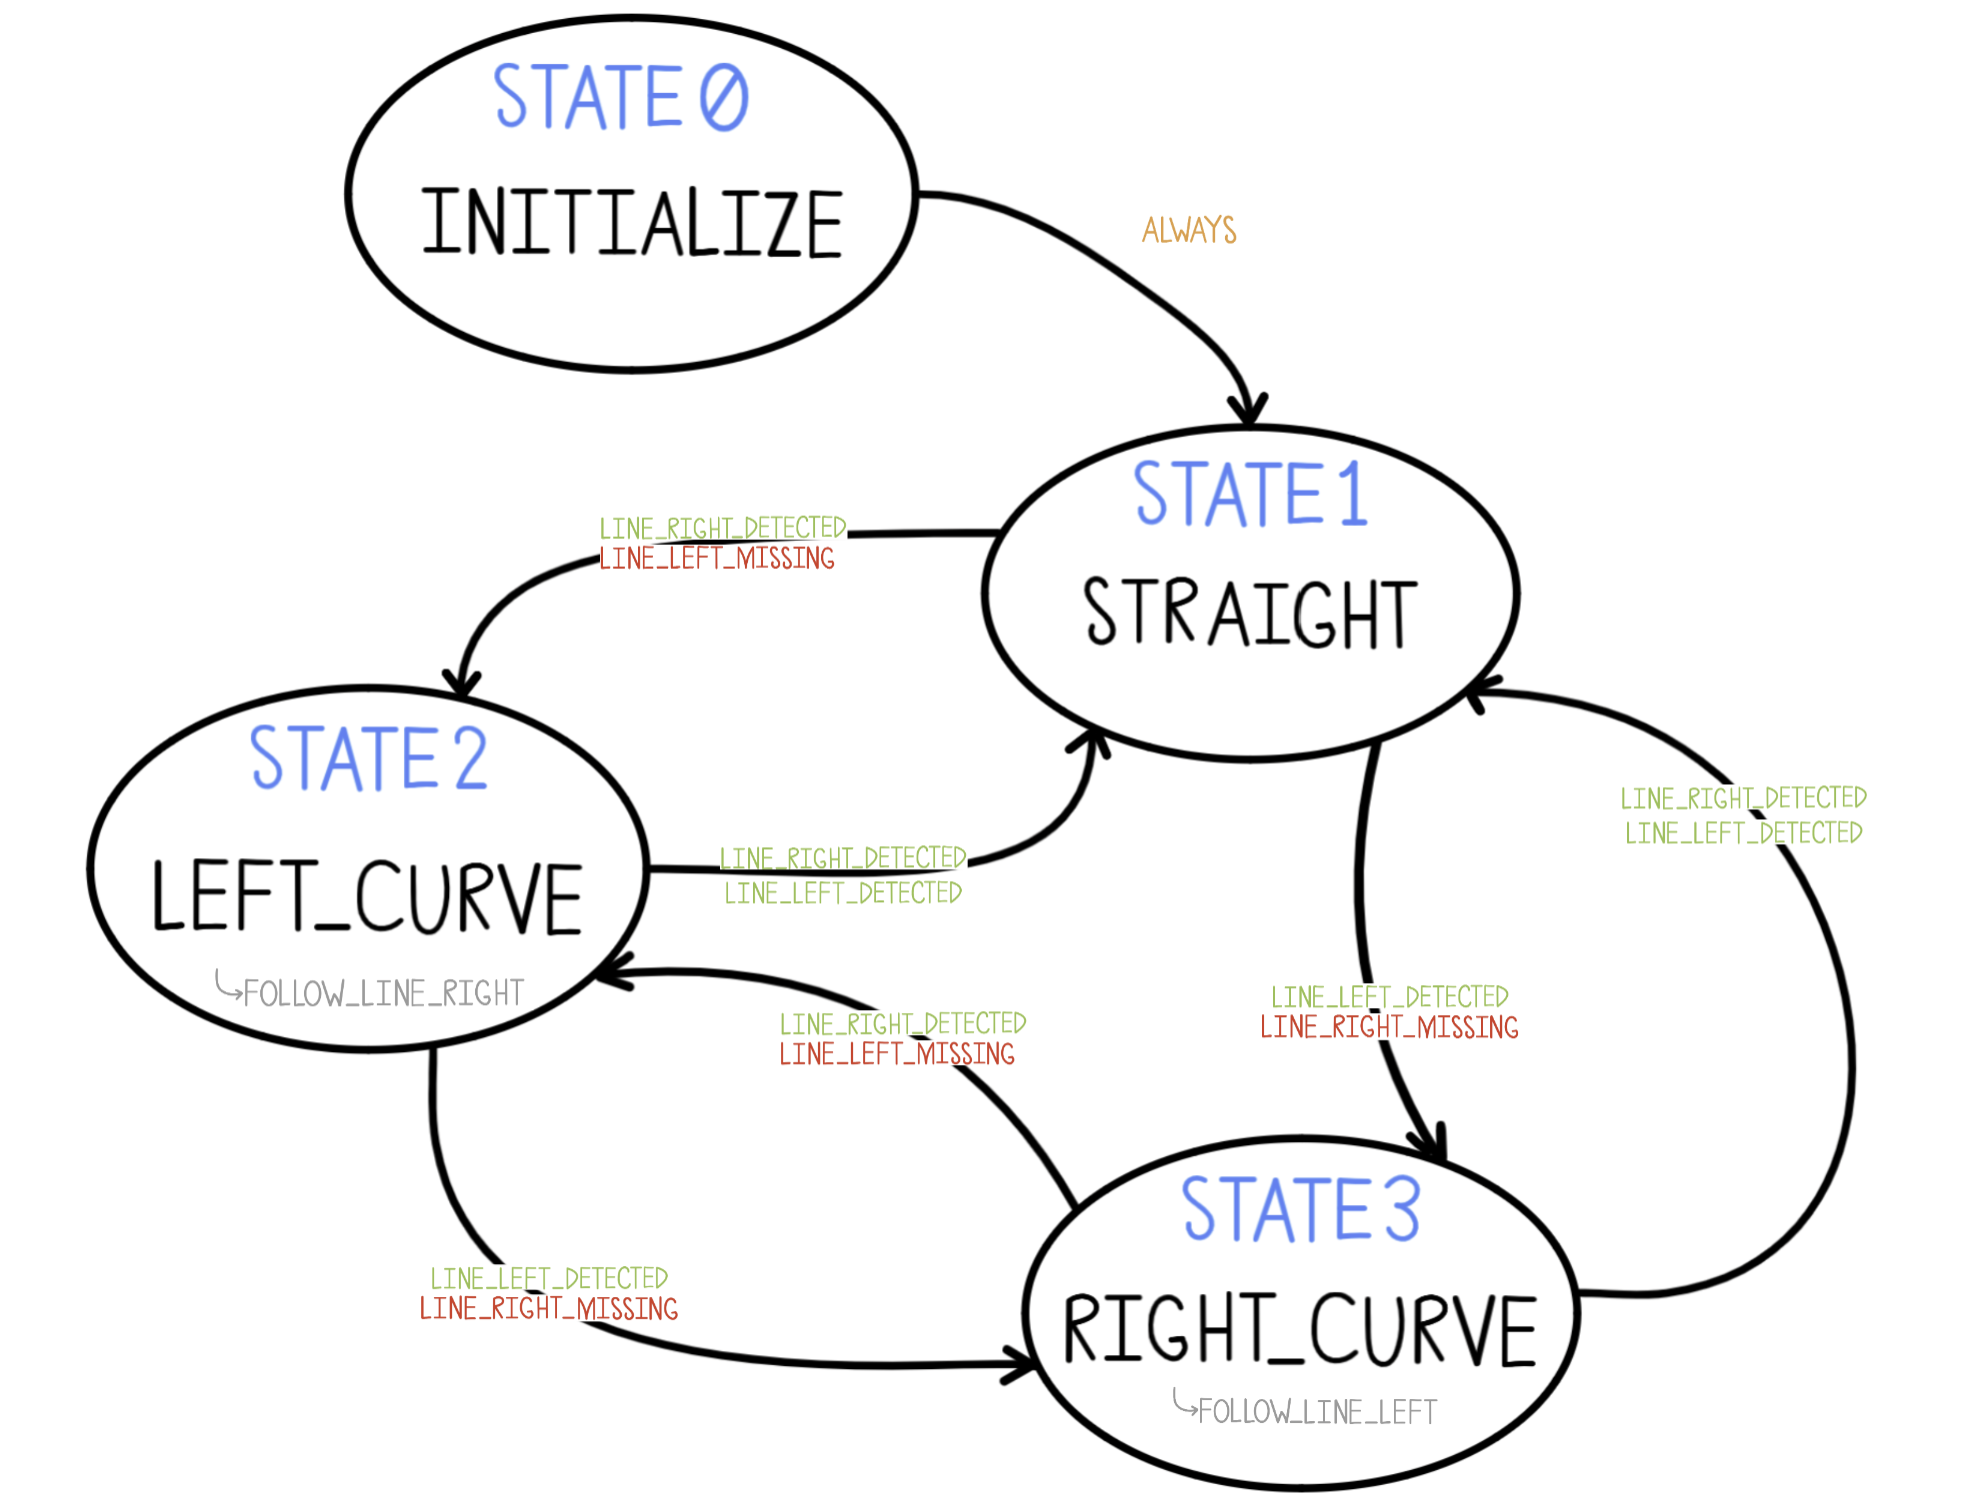
\includegraphics[width=5.92in,height=4.05in,keepaspectratio]{FSM_Diagram.png}};

% tight explanatory block
\fill[SoftGreen,rounded corners=3pt]
($(current page.north west)+(6.66in,-2.10in)$)
rectangle
($(current page.north west)+(10.54in,-5.95in)$);

\node[
    anchor=north west,
    align=left,
    text width=2.95in,
    font=\fontsize{6.95}{6.45}\selectfont,
    text=Ink
]
at ($(current page.north west)+(6.90in,-2.35in)$)
{
\textbf{\textcolor{DeepGreen}{STATE 0 — INITIALIZE}}\\
Establish controller variables, then enter normal driving.\\[5pt]

\textbf{\textcolor{DeepGreen}{STATE 1 — STRAIGHT}}\\
Both lane boundaries are available.\\[5pt]

\textbf{\textcolor{DeepGreen}{STATE 2 — LEFT\_CURVE}}\\
Left boundary missing; use \texttt{LINE\_RIGHT}.\\[5pt]

\textbf{\textcolor{DeepGreen}{STATE 3 — RIGHT\_CURVE}}\\
Right boundary missing; use \texttt{LINE\_LEFT}.\\[6pt]

\textbf{\textcolor{DeepGreen}{TRANSITION VARIABLES}}\\
\texttt{LINE\_LEFT\_DETECTED}\\
\texttt{LINE\_RIGHT\_DETECTED}
};

% steering response — text and plot positions switched for better balance
\node[
    anchor=north west,
    text=DeepGreen,
    font=\sffamily\bfseries\fontsize{8.3}{7.4}\selectfont
]
at ($(current page.north west)+(0.46in,-6.35in)$)
{STEERING RESPONSE};

% PD controller explanation now occupies the left column
\node[
    anchor=north west,
    align=left,
    text width=4.10in,
    font=\fontsize{7.35}{8.35}\selectfont,
    text=Ink
]
at ($(current page.north west)+(0.46in,-6.74in)$)
{
A \textbf{PD steering controller} translated the selected visual reference
into a steering command. Offline comparison against recorded steering data
provided a way to tune proportional and derivative behavior before physical
testing.
};

% Steering-response plot: original size restored.
% The image is physically moved so its rendered right edge aligns with
% the right edge of the light-green state-description panel above.
\node[
    anchor=north east,
    inner sep=0pt
]
at ($(current page.north west)+(10.54in,-6.11in)$)
{
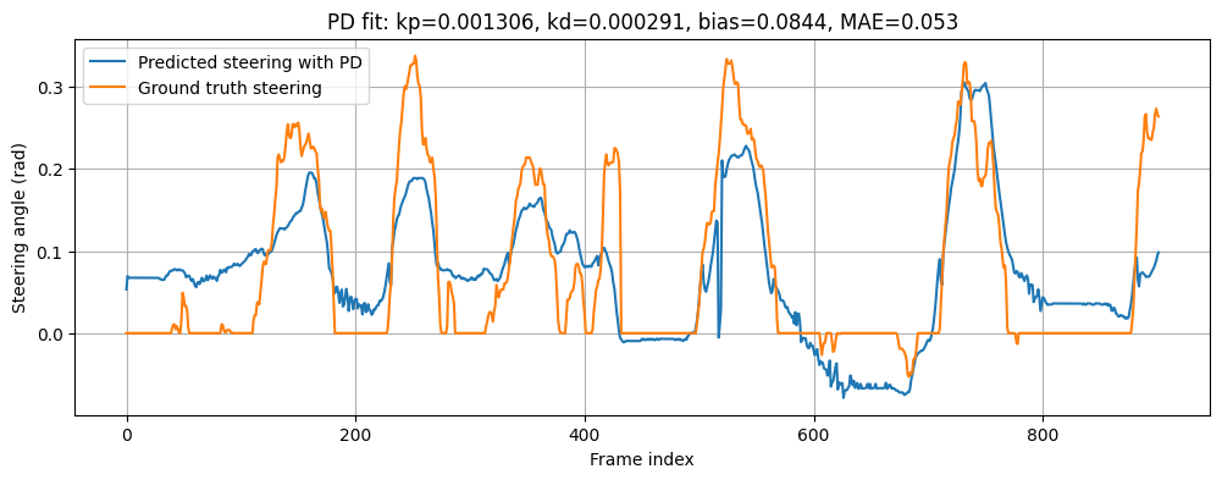
\includegraphics[
    width=6.40in,
    height=1.92in,
    keepaspectratio
]{FSM_PDcontroller.png}
};

\RFFooter
{\hyperlink{roadfollowing-state}{\faArrowLeft\ ROAD STATE}}
{8 / 9}
{\hyperlink{roadfollowing-result}{PHYSICAL RESULT \faArrowRight}}

\end{tikzpicture}


%==============================================================
% PAGE 11H — PHYSICAL VALIDATION
%==============================================================

\clearpage
\thispagestyle{empty}
\hypertarget{roadfollowing-result}{}
\null

\begin{tikzpicture}[remember picture,overlay]

\RFPageBase
\RFHeader
{PHYSICAL VALIDATION}
{AUTONOMOUS ROAD FOLLOWING}
{Physical course validation
\hspace{7pt}\textbullet\hspace{7pt}
full-loop completion
\hspace{7pt}\textbullet\hspace{7pt}
integrated perception--decision--control}

% -------------------------------------------------------------
% HERO — restored to full page-threshold width
% Cropped slightly at top/bottom so the bottom content still fits.
% -------------------------------------------------------------
\node[
    anchor=north west,
    inner sep=0pt,
    draw=DeepGreen,
    line width=0.85pt
]
at ($(current page.north west)+(0.46in,-1.76in)$)
{
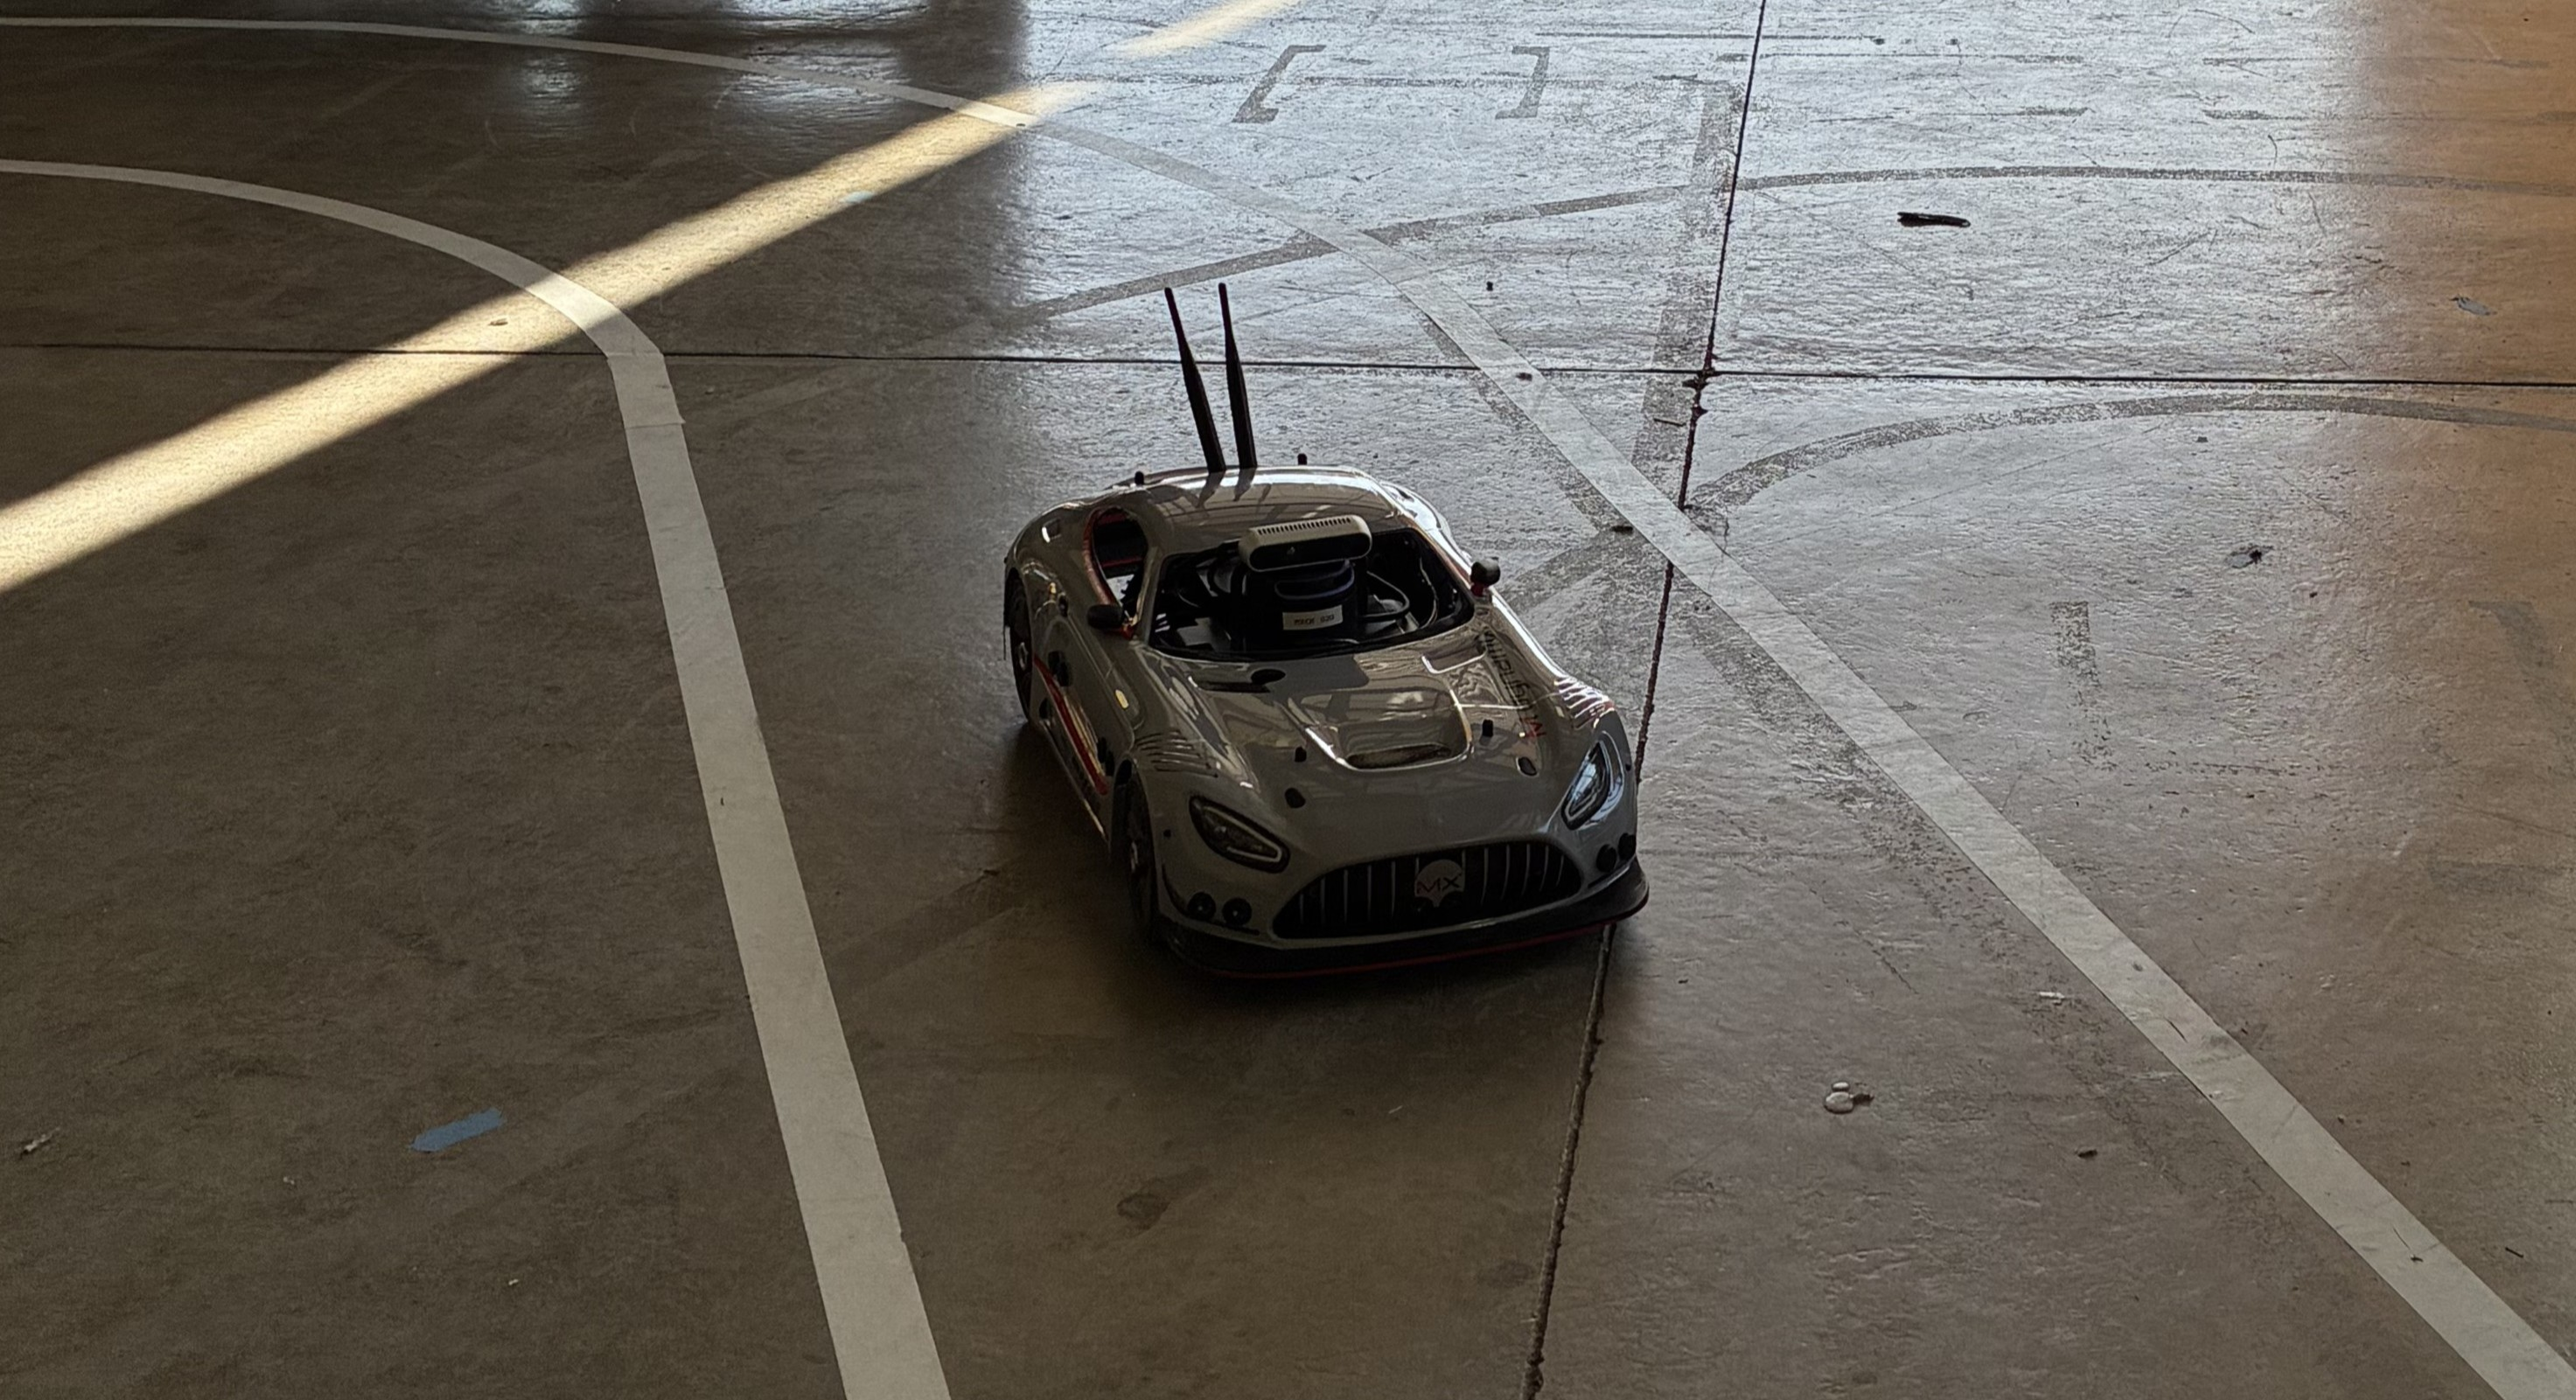
\includegraphics[
    width=10.08in,
    trim=0 78bp 0 78bp,
    clip
]{car_hero.jpg}
};

% Tight banner on image
\node[
    anchor=south west,
    fill=DeepGreen,
    text=white,
    inner xsep=8pt,
    inner ysep=4pt,
    font=\sffamily\bfseries\fontsize{7.0}{7.7}\selectfont
]
at ($(current page.north west)+(0.62in,-6.5in)$)
{PHYSICAL AUTONOMOUS VEHICLE PLATFORM};

% -------------------------------------------------------------
% BOTTOM CONTENT — cleaner two-column case-study closeout
% -------------------------------------------------------------

% Left outcome block
\node[
    anchor=north west,
    text=DeepGreen,
    font=\sffamily\bfseries\fontsize{8.25}{9.0}\selectfont
]
at ($(current page.north west)+(0.46in,-6.84in)$)
{PROJECT OUTCOME};

\draw[PolyGold,line width=1.15pt]
($(current page.north west)+(0.46in,-7.02in)$) --
($(current page.north west)+(5.95in,-7.02in)$);

\node[
    anchor=north west,
    align=left,
    text width=5.45in,
    font=\fontsize{6.55}{7.45}\selectfont,
    text=Ink
]
at ($(current page.north west)+(0.46in,-7.00in)$)
{
The completed road follower autonomously navigated a full loop of the course.
The project demonstrated an iterative robotics workflow: analyze recorded
sensor data, prototype perception algorithms, identify failure modes,
restructure the decision logic, tune control behavior, and validate the
complete system on hardware.\\[4pt]
The final architecture remained modular: perception generated lane evidence,
the FSM interpreted local road geometry, and the steering controller converted
that decision into vehicle motion.
};

% Right methods block
\fill[SoftGreen!68,rounded corners=4pt]
($(current page.north west)+(6.40in,-6.82in)$)
rectangle
($(current page.north west)+(10.54in,-7.94in)$);


% CORE METHODS label intentionally drawn AFTER the panel so it stays visible
% and appears in front of the SoftGreen fill.
\node[
    anchor=north west,
    text=DeepGreen,
    font=\sffamily\bfseries\fontsize{8.25}{9.0}\selectfont
]
at ($(current page.north west)+(6.66in,-6.84in)$)
{CORE METHODS};

\node[
    anchor=north west,
    align=left,
    text width=3.72in,
    font=\fontsize{6.35}{7.10}\selectfont,
    text=Ink
]
at ($(current page.north west)+(6.66in,-7.00in)$)
{
\textbf{PERCEPTION + CONTROL}\\[-1pt]
Python \hspace{5pt}\textbullet\hspace{5pt}
Computer Vision \hspace{5pt}\textbullet\hspace{5pt}
Canny Edge Detection\\
ROI + Image Masking \hspace{5pt}\textbullet\hspace{5pt}
Finite-State Machines\\
PD Feedback Control \hspace{5pt}\textbullet\hspace{5pt}
Offline Data Analysis\\[5pt]

\textbf{\textcolor{DeepGreen}{PLATFORM + TOOLS}}\\[-1pt]
NVIDIA Jetson \hspace{5pt}\textbullet\hspace{5pt}
Intel RealSense\\
Google Colab \hspace{5pt}\textbullet\hspace{5pt}
Foxglove
};

\RFFooter
{\hyperlink{roadfollowing-fsm}{\faArrowLeft\ FSM + CONTROL}}
{9 / 9}
{PROJECT 12 \faArrowRight}

\end{tikzpicture}



%\clearpage